\graphicspath{{8analytic/pics/}}
\section{Analytic Geometry and Calculus}

\subsection{Axes and Co-ordinates}

Modern mathematics is almost entirely \emph{algebraic}: we trust equations and the rules of algebra more than pictures. For example, modern mathematics considers the expression $(x+y)^2=x^2+2xy+y^2$ to follow from the laws (axioms) of algebra:
\begin{align*}
	(x+y)^2&=(x+y)(x+y)\tag*{(definition of `square')}\\
	&=x(x+y)+y(x+y)\tag*{(distributive law)}\\
	&=x^2+xy+yx+y^2\tag*{(distributive law twice more)}\\
	&=x^2+2xy+y^2\tag*{(commutativity)}
\end{align*}
\begin{minipage}[t]{0.72\linewidth}\vspace{0pt}
	For most of mathematical history, this result would have been viewed \emph{geometrically} as in Euclid's \emph{Elements} (Thm II.\,4):
	\begin{quote}
		The square on two parts equals the squares on each part plus twice the rectangle on the parts.
	\end{quote}
	The proof was a simple picture.
\end{minipage}
\hfill
\begin{minipage}[t]{0.25\linewidth}\vspace{0pt}
	\flushright
\includegraphics{analytic-euclid}
\end{minipage}
\smallbreak

We've seen how algebra and algebraic notation were slowly adopted in renaissance Europe. While its utility for efficient calculation was noted, algebra was not initially considered acceptable for \emph{proof} and calculations would be justified geometrically. From our modern viewpoint this seems backwards: if a student today were asked to prove Euclid's result, they'd likely label the `parts' $x$ and $y$, before using the algebraic formula at the top of the page to justify the result! Of course each line in the algebraic proof has a geometric basis:
\begin{itemize}
  \item Distributivity says that the rectangle on a side and two parts equals the sum of the rectangles on the side and each of the parts respectively.
  \item Commutativity says that a rectangle has the same area if rotated \ang{90}.
\end{itemize}
Modern mathematics has converted geometric rules into algebra and largely forgotten their geometric origin! This slow movement from geometry to algebra is one of the great revolutions of mathematical history, completely changing the way mathematicians \emph{think.} More practically, the conversion to algebra allows easier generalization: how would one geometrically justify an expression such as
\[
	(x+y)^4=x^4+4x^3y+6x^2y^2+4xy^3+y^4\text{ ?}
\]
Euclidean Geometry is \emph{synthetic:} based on purely geometric axioms without formulæ or co-ordinates. The revolution of \emph{analytic geometry} was to marry algebra and geometry using \emph{axes} and \emph{co-ordinates.} Modern geometry is primarily analytic and it is now rare to find a mathematician working solely in synthetic geometry---algebra's domination of Euclidean geometry is total! The critical step in this revolution was made almost simultaneously by two Frenchmen\ldots
\goodbreak


\boldinline{Pierre de Fermat (1601--1665)} Mathematics was Fermat's pastime rather than his profession, though this didn't prevent him making great strides in several areas such as probability, analytic geometry, early calculus, number theory and optics.\footnote{%
	Fermat was wealthy but not aristocratic, attending the University of Orléans for three years where he trained as a lawyer. You've likely encountered his name in relation to two famous results in number theory: 
	\begin{description}
		\item[\normalfont\emph{Fermat's Little Theorem}] $p$ prime $\Longrightarrow x^p\equiv x\pmod p$ for all integers $x$.
		\item[\normalfont\emph{Fermat's Last Theorem}] If $n\in\N_{\ge 3}$, then $x^n+y^n=z^n$ has no integer solutions with $xy z\neq 0$. Fermat is not believed to have proved this beyond a special case ($n=4$), with a complete proof not appearing until the 1990s. 
	\end{description}
} Some of Fermat's fame comes from his enigma, with most of what we know of his work coming in letters to friends in which he rarely offers proofs. He would regularly challenge friends to prove results, and it is often unknown whether he had proofs himself or merely suspected a general statement. Being outside the mainstream, his ideas were often ignored or downplayed. When he died, his notes and letters contained many unproven claims. Leonhard Euler (1707--1783) in particular expended much effort proving several of these.\smallbreak
Fermat's approach to analytic geometry was not dissimilar to that of Descartes which we shall describe below: he introduced a single axis which allowed the conversion of curves into algebraic equations. We'll return to Fermat when we discuss the beginnings of calculus in the next section.


\boldinline{René Descartes (1596--1650)} In his approach to mathematics, Descartes is the chalk to Fermat's cheese, rigorously recording everything. His defining work is 1637's \emph{Discours de la méthode\ldots}\footnote{\ldots \emph{of rightly conducting one's reason and of seeking truth in the sciences.} The primary part of this work is philosophical and contains his famous phrase \emph{cogito egro sum} (\emph{I think therefore I am}).} While enormously influential in philosophy, \emph{Discours} was intended to lay the groundwork for investigation within mathematics and the sciences---Descartes finishes \emph{Discours} by commenting on the necessity of experimentation in science and on his reluctance to publish due to the environment of hostility surrounding Galileo's prosecution.\footnote{At this time, France was still Catholic. Descartes had moved thence to Holland in part to pursue his work more freely. In 1649 Descartes moved to Sweden where he died the following year.} The copious appendices to \emph{Discours} contain Descartes' scientific work. It is in one of these, \emph{La Géométrie,} that Descartes introduces axes and co-ordinates.
\par


\begin{minipage}[t]{0.64\linewidth}\vspace{0pt}
	We now think of Cartesian axes and co-ordinates as \emph{plural,} but both Fermat and Descartes used only one axis. Here is a sketch of their approach.
	\smallbreak
	Draw a straight line (the \textcolor{red}{axis}) containing two fixed points labelled 0 (the \emph{origin}) and 1. All points on the axis are identified with numbers $x$ (originally only positive).
	\smallbreak
	A \textcolor{blue}{curve} is described as an algebraic relationship between \textcolor{red}{$x$} and the \textcolor{Green}{distance $y$} from the axis to the curve measured using a family of \textcolor{Green}{parallel lines} intersecting both. 
\end{minipage}
\hfill
\begin{minipage}[t]{0.35\linewidth}\vspace{0pt}
	\flushright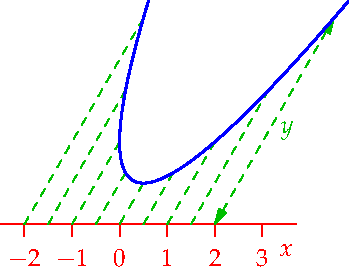
\includegraphics{analytic-parab}
\end{minipage}
\medbreak

Neither Descartes nor Fermat had a second axes, though their approach implicitly imagines one, the \textcolor{Green}{measuring line} through the origin. It therefore makes sense for us to speak of the \emph{co-ordinates} $(x,y)$; the modern terms \emph{abscissa} ($x$) and \emph{ordinate} ($y$) date from shortly after the time of Descartes. It wasn't long before a second axis orthogonal to the first was instituted (Frans van Schooten, 1649), an approach that quickly became standard.
\goodbreak


\boldinline{Example 1} The previous picture shows some of the flexibility in Descartes' approach. The curve $y=x^2+1$ is drawn, where the `$y$-axis' is inclined \ang{60} to the horizontal. To recognize the curve in a more standard fashion, we can perform a change of co-ordinates. Suppose $P=(x,y)$ with respect to the slanted axes and $(X,Y)$ with respect to the usual orthogonal axes.
\begin{center}
	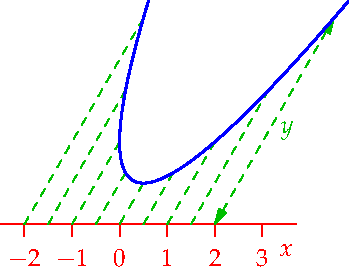
\includegraphics{analytic-parab}
	\qquad\qquad
	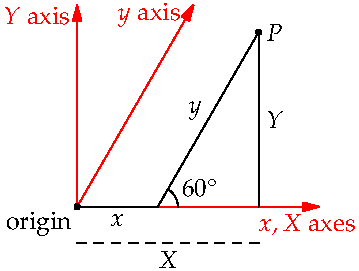
\includegraphics{analytic-parab2}
\end{center}
The second picture shows that
\[
	\begin{cases}
		X=x+y\cos \ang{60}=x+\frac 12y \\
		Y=y\sin \ang{60}=\frac{\sqrt 3}2y
	\end{cases}
\]
For any point on the curve,
\begin{align*}
	\sqrt 3X-Y=\sqrt 3x&\implies (\sqrt 3X-Y)^2=3x^2=3(y-1)=3\left(\frac 2{\sqrt 3}Y-1\right)\\
	&\implies 3X^2-2\sqrt 3 XY+Y^2-2\sqrt 3Y+3=0
\end{align*}
which is an implicit equation for a parabola.\footnote{%
	This really is a parabola, just rotated! This may be confirmed by computing its \emph{discriminant}: a non-degenerate quadratic curve $aX^2+bXY+cY^2+\text{linear terms}$ is a parabola if and only if $b^2-4ac=0$.
}


\boldinline{Example 2} Analytic geometry affords easy proofs of many results that are significantly harder in Euclidean geometry. For instance, here is the famous \emph{centroid theorem.}
\par
\begin{minipage}[t]{0.68\linewidth}\vspace{-5pt}
	Choose axes pointing along two sides of a triangle with the origin at one vertex.
	\par
	If the two axes-side lengths are $a$ and $b$, then the third side has equation $bx+ay=ab$ or $y=b-\frac bax$ and the midpoints of the sides have co-ordinates as in the picture. Now compute the point 1/3 of the way along each median: for instance
	\[
		\frac 23\left(\frac a2,0\right)+\frac 13(0,b)=\frac 13(a,b)
	\]
	One obtains the same result with the other medians, whence \emph{all three meet at a common point} $G$, the \emph{centroid} of the triangle.
\end{minipage}
\hfill
\begin{minipage}[t]{0.3\linewidth}\vspace{-15pt}
	\flushright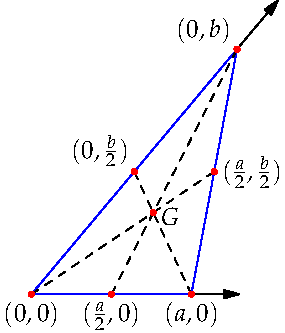
\includegraphics{analytic-centroid}
\end{minipage}
\medbreak


This ability to \emph{choose axes to fit the problem} is a critical advantage of analytic geometry, largely dispensing with the tedious consideration of \emph{congruence} in synthetic geometry.

\smallbreak

Descartes used his method to solve problems that had proved more difficult synthetically, such as finding complicated intersections of curves. As we'll see in the next section, such arguments would often rely on his Factor Theorem (pg.\,\pageref{pg:factorthm}). Given the novelty of his approach, Descartes typically gave geometric proofs of all assertions to back up his algebraic work. However he also saw the future, stating that once several examples were done it was no longer necessary to draw physical lines and provide a geometric argument, \emph{the algebra was the proof.}




\begin{exercises}{}{}
	\exstart %[14]
	Assume that $xy=c$ represents a hyperbola with asymptotes the $x$- and $y$-axes. Show that $xy+c=rx+sy$ also represents a hyperbola, and find its asymptotes.
	\begin{enumerate}\setcounter{enumi}{1}
	  \item%[14-10] 
	  Determine the locus of the equation $b^2-2x^2=2xy+y^2$.\par
	  (\emph{Hint: add $x^2$ to both sides and remember that `axes' do not have to be orthogonal\ldots})
	  
	  \item%[14-14]*
	  We describe a method whereby Descartes constructed the product of two lengths.\par
	  \begin{minipage}[t]{0.68\linewidth}\vspace{-5pt}
		  \begin{quote}
		  	Let $\ray{BC}$ and $\ray{BD}$ be rays forming an acute angle at $B$. Our goal is to multiply $\nm{BD}$ by $\nm{BC}$.\par
		  	Suppose $\nm{AB}=1$, where $A$ lies on $\ray{BD}$. \par
		  	Join $\cl{AC}$ and draw $\cl{DE}$ parallel to $\cl{AC}$ so that $E\in\ray{BC}$.
		  \end{quote}
		  Prove that $\nm{BE}$ is the product of $\nm{BD}$ and $\nm{BC}$.
	  \end{minipage}
	  \hfill
	  \begin{minipage}[t]{0.31\linewidth}\vspace{-10pt}
	  	\flushright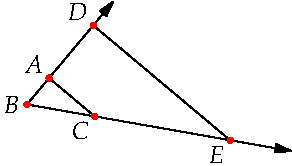
\includegraphics{descartes-product}
	  \end{minipage}
	  \smallbreak
	  Similarly, given lengths $\nm{BE}$ and $\nm{BD}$, construct a segment whose length is the quotient $\frac{\nm{BE}}{\nm{BD}}$.
	  
	  \item Here is a geometric justification of Descartes for the solution of the equation $x^2=ax+b^2$, where $a,b>0$.
	  \par
		\begin{minipage}[t]{0.6\linewidth}\vspace{-5pt}
			\begin{itemize}\itemsep0pt
			  \item Let $\cl{OQ}$ and $\cl{PQ}$ be perpendicular with lengths $\frac a2$ and $b$ respectively.
			  \item Draw the circle centered at $O$ with radius $\frac a2$.
			  \item Draw and extend the line $\lin{OP}$.
			  \item The solution is $x=\nm{NP}$.
			\end{itemize}
		\end{minipage}
		\hfill
		\begin{minipage}[t]{0.35\linewidth}\vspace{-10pt}
			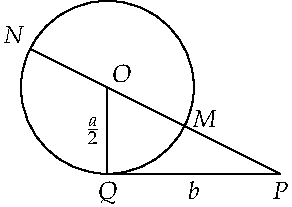
\includegraphics{descartes-quad}
		\end{minipage}\par
		\begin{enumerate}
		  \item Prove that Descartes' construction indeed recovers a solution.
	  
		  \item Show that the other solution to the equation $x^2=ax+b^2$ is negative (\emph{false} to Descartes). How is it visible in the picture?
	  	
		  \item Explain how the same picture could be used to solve the equation $x^2+ax=b^2$.
		\end{enumerate}
	\end{enumerate}
\end{exercises}


% EDIT picture in 4 to be more like quiz.
% 
% Add question.
% \item Fermat, following the work of Islamic mathematicians such as Omar Khayyam, was able to describe the solutions to certain cubic equations as the intersection of two conics. For example, to solve $x^3+bx^2=bc$ (where $b,c>0$), he would introduce a new variable $y$ setting both sides equal to $b xy$. The (positive) solution is then the $x$-solution to the system of equations
% \[
% 	\begin{cases}
% 		x^2+bx=by\\
% 		xy=c
% 	\end{cases}
% \]
% Sketch these curves explicitly for the example $x^3+4x^2=24$

\clearpage



\subsection{The Beginnings of Calculus}\label{sec:calc1}

At the heart of calculus is the relationship between \emph{velocity, displacement, rate of change} and \emph{area.}
\begin{itemize}\itemsep0pt
  \item The \emph{instantaneous velocity} of a particle is the \emph{rate of change} of its \emph{displacement.}
  \item The \emph{displacement} of a particle is the \emph{net area} under its \emph{velocity-time} graph.
\end{itemize}
To state these principles requires graphs. Analytic geometry makes computation much easier (\emph{rate of change} means \emph{slope}). Once it appeared in the early 1600s, the rapid development of calculus was arguably inevitable. However, many of the basic ideas long predate Descartes and Fermat.\smallbreak
In the context of the above principles, the \emph{Fundamental Theorem of Calculus} is intuitive: complete knowledge of displacement (from some starting point) is equivalent to complete knowledge of velocity. The modern statement is more daunting, though familiar:

\begin{thm*}{}{}
	\exstart If $f$ is continuous on $[a,b]$, then $F(x):=\int_a^xf(u)\,\du$ is continuous on $[a,b]$, differentiable on $(a,b)$, and $F'(x)=f(x)$.
	\begin{enumerate}\setcounter{enumi}{1}
	  \item If $F$ is continuous on $[a,b]$ with integrable derivative on $(a,b)$, then $\int_a^bF'(x)\,\dx=F(b)-F(a)$.
	\end{enumerate}
\end{thm*}

The triumph of the modern version is its abstraction and wide applicability: we've gone way beyond considerations of velocity ($f$) and displacement ($F$). The challenge of \emph{teaching}\footnote{Calculus students can easily be taught the mechanics of calculus (the power law, chain rule, etc.) without having any idea of its meaning; witness the power and curse of analytic geometry and algebra!} and \emph{proving} the Fundamental Theorem lies in developing and understanding what is meant by \emph{continuous, differentiable} and \emph{integrable.} The quest for good definitions of these concepts is the story of analysis in the 17-1800s. We begin with some older considerations of the velocity and area problems.


\boldsubsubsection{The Velocity Problem pre-1600}

The modern ideas of \emph{uniform/average} velocity are straightforward:
\begin{quote}
Measure how far an object travels in a given time interval and divide one by the other.
\end{quote}
While several ancient Greek mathematicians %(e.g.\ Autolycus)
considered this (and uniform acceleration), the challenge of considering a ratio of two unlike quantities (distance\,:\,time) proved difficult to surmount. Around 1200, Gerard of Brussels resurrected this approach as a definition of velocity, though it was not  considered a numerical quantity in its own right.\smallbreak

Gerard was credited in the 1330s by the Oxford/Merton Thinkers %\footnote{Or Merton Thinkers, based at Merton College, Oxford. They included Thomas Bardwardine, William Heytesbury, etc.}
as influencing their investigations of \emph{instantaneous velocity,} a much more difficult issue. They offered the following definition and made the first statement of the `mean speed theorem,' though both are vague and logically dubious.

\begin{defn*}{}{}
The \emph{velocity} of a particle at an instant will be measured as the uniform velocity along the path that would have been taken by the particle if it continued with that velocity.
\end{defn*}

This is really a convoluted idea of inertial motion.

\begin{thm*}{}{}
If a particle is uniformly accelerated from rest to some velocity, it will travel half the distance it would have traveled over the same interval with the final velocity.
\end{thm*}

For centuries it was thought that Galileo was the first to state such ideas (compare his falling body discussion, pg.\,\pageref{pg:galileo}), but the Oxford group beat him by 250 years. They had no algebra with which to prove their assertions and essentially only asserted examples. %Indeed the best they could manage was to assert the proportion of powers rule: if time intervals are in the proportion $2:1$ and if particles subject to the same uniform acceleration are accelerated from rest over these intervals, then the resulting distances traveled will be in the proportion $4:1$. In modern notation:
%\[v_1=at,\quad v_2=2at\implies d_1=\frac 12v_1t=\frac 12at^2,\quad d_2=\frac 12v_2\cdot 2t=2at^2=4d_2\]
\smallbreak
In the 1350's, Nicolas Oresme (Paris) considered velocity geometrically by (essentially) drawing velocity-time graphs. As we saw previously, this is essentially the approach taken by Galileo; it is also an early version of \emph{axes.} A major difference is that Galileo married mathematics to \emph{observation}; uniform acceleration for Galileo was precisely the motion of a falling body.
\smallbreak


A proper definition of \emph{instantaneous velocity} is difficult because it requires \emph{limits,} measuring average velocity over smaller and smaller intervals. You are in good company if you find this challenging: Zeno's arrow paradox is essentially an objection to the very idea of instantaneous velocity! Even if one accepts the concept, its direct measurement, even in modern times, is essentially impossible.\footnote{%
	For instance, radar Doppler-shift (as used to catch speeding motorists) requires measuring the wavelength of a radar beam, which essentially compute the average velocity over a very small time interval. %Indeed quantum mechanics suggests that instantaneous velocity and precise location are possibly meaningless concepts. Thankfully mathematicians can choose to deal with idealized models of the universe rather than the real thing!
}


\boldsubsubsection{The Area Problem pre-1600}

We've previously seen two situations in which calculus-like methods were used to describe areas.
\begin{itemize}
  \item Archimedes (sec.\,\ref{sec:archimedes}) computed/approximated the area of a circle and inside a parabola using infinitely many triangles. His `cross-section' approach to finding area and volume also seems modern, though this work remained unknown until 1899.
  \item Kepler (pg.\,\pageref{pg:kepler2}) argued for his second law (equal areas in equal times) using infinitesimally small triangles to approximate segments of an ellipse. He also applied this method to several other problems, crediting Archimedes with the approach.
\end{itemize}

The modern notion of Riemann sums is just a special case of approximating an area using small rectangles: the philosophical challenge is again the notion of \emph{limits} and infinitesimals.\par
\begin{minipage}[t]{0.58\linewidth}\vspace{-3pt}
	In an early antecedent, Oresme describes how to compute the distance travelled by a particle whose speed is constant on a sequence of intervals. For example:\smallbreak
	Over the time interval $\left[\tfrac 1{2^{n+1}},\tfrac 1{2^n}\right)$ a particle travels at speed $1+3n$. How far does it travel in 1 second?\smallbreak
	Oresme drew boxes to compute areas and obtain
	\[
		d=\sum_{n=0}^\infty(1+3n)\left(\frac 1{2^n}-\frac 1{2^{n+1}}\right) =\sum_{n=0}^\infty \frac{1+3n}{2^{n+1}}=4
	\]
	Similar to Archimedes, the infinite sum was evaluated by spotting two patterns:
\end{minipage}
\hfill
\begin{minipage}[t]{0.4\linewidth}\vspace{-3pt}
	\flushright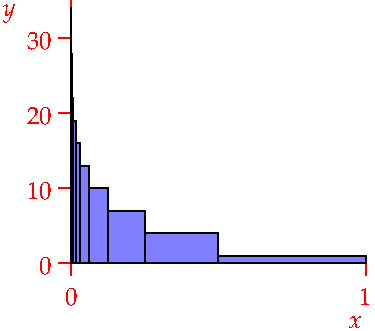
\includegraphics{analytic-oresme}
\end{minipage}\par
\begin{gather*}
	\frac 12+\frac 1{2^2}+\frac 1{2^3}\cdots+\frac 1{2^{n+1}}=1-\frac 1{2^{n+1}}
	\qquad\qquad
	\frac 02+\frac 1{2^2}+\frac 2{2^3}+\frac 3{2^4}+\cdots+\frac n{2^{n+1}}=1-\frac{n+2}{2^{n+1}}
\end{gather*}
Oresme had neither our notation nor our (limit-dependent) concept of an infinite series! He also worked with similar problems for uniform accelerations over intervals. These are not true Riemann sums, nor are they physical, for a particle cannot suddenly change speed!
\goodbreak


\boldsubsubsection{Calculus à la Fermat \& Descartes}

The advent of analytic geometry allowed Fermat and Descartes to turn the computation of instantaneous velocity and related differentiation problems into algebraic processes. The velocity of an object is now identified with the slope of the displacement-time graph, which can be computed using variations on the modern method of \emph{secant lines.} We discuss their competing methods.

\begin{minipage}[t]{0.63\linewidth}\vspace{0pt}
	\boldinline{Fermat's method of adequation}
	
	Consider the function $p(x)=x^3-12x+19$; the goal is to find the minimum, which we know to be located at the $x$-value $m=2$.\par
	Fermat argues that if $x_1,x_2$ are located near $m$ such that $p(x_1)=p(x_2)$, then the polynomial $p(x_2)-p(x_1)$ (which equals zero!) is divisible by $x_2-x_1$. Indeed
	\begin{align*}
		0&=\frac{p(x_2)-p(x_1)}{x_2-x_1}\\
		&=\frac{x_2^3-12x_2+19-x_1^3+12x_1-19}{x_2-x_1}\\
		&=\frac{(x_2-x_1)(x_2^2+x_1x_2+x_1^2-12)}{x_2-x_1}\\
		&=x_2^2+x_1x_2+x_1^2-12
	\end{align*}
\end{minipage}
\hfill
\begin{minipage}[t]{0.35\linewidth}\vspace{0pt}
	\flushright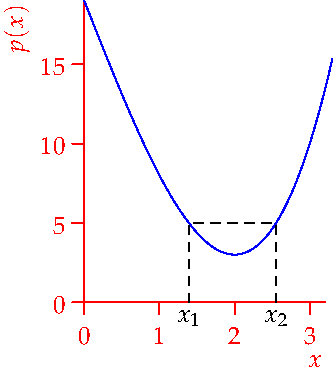
\includegraphics{analytic-adequation}
\end{minipage}\medbreak

Since this holds for any $x_1,x_2$ with $p(x_1)=p(x_2)$, Fermat claims it also holds when $x_1=x_2=m$ (note the assumption of continuity!), and he concludes
\[
	3m^2-12=0\implies m=2
\]
By considering values of $x$ near $m$, it is clear that Fermat really has found a local minimum. We recognize the idea that the slope of the tangent line is zero at local extrema.
\smallbreak

This approach dates from the 1620s and is similar to earlier work of Viète. Fermat later alters his method by considering values $p(x)$ and $p(x+e)$ for small $e$ ($x$ is `adequated by $e$'). The difference $p(x+e)-p(x)$ is more easily divided by $e$ without factorizing. Compared with the above, we obtain
\begin{align*}
	0&=\frac{p(x+e)-p(x)}{e} =\frac{x^3+3x^2e+3xe^2+e^3-12x-12e+19-x^3+12x-19}{e}\\
	&=\frac{3x^2e+3xe^2+e^3-12e}{e} =3x^2-12 +3xe+e^2
\end{align*}
Fermat finished by setting $e$ to zero and solving for $x$ as before. Observe the derivative $p'(x)=3x^2-12$ and how $e$ plays the role of $h$ in the modern expression
\[
	p'(x)=\lim_{h\to 0}\frac{p(x+h)-p(x)}h
\]
Fermat's method works for any polynomial, where the limit definition of derivative requires no more than simple evaluation at $h=0$. Fermat also extended his method to cover implicit curves and their tangents.
\goodbreak


\boldinline{Descartes' method of normals}\phantomsection\label{pg:descartesnormal}

Descartes and Fermat are known to have corresponded regarding their methods. Descartes indeed seems to have felt somewhat challenged by Fermat, and engaged in some criticism of his approach. Descartes' method (in \emph{La Géométrie}) relies on circles and repeated roots of polynomials in order to compute tangents.\smallbreak

In this example, we compute the slope of the curve \textcolor{blue}{$y=\frac 14(10x-x^2)$} at the point $P=(4,6)$.
\begin{center}
	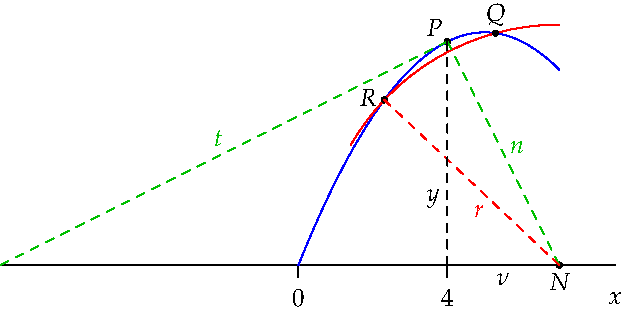
\includegraphics[scale=0.9]{analytic-desnormal}
\end{center}
Let $N=(4+\nu,0)$ be where the \textcolor{Green}{normal} to the curve intersects the $x$-axis.\footnote{%
	At the time, $\nu$ was known as the \emph{subnormal} and $t$ the \emph{tangent.}
}
Draw a \textcolor{red}{circular arc} radius $r$ centered at $N$.
If $r$ is close to $n$, the circle intersects the curve in two points $Q,R$ near to $P$. The line $\lin{QR}$ plainly approximates the tangent at $P$.
\smallbreak
The co-ordinates of $Q,R$ may be found by solving algebraic equations: substituting $y=\frac 14(10x-x^2)$ into the equation for the circle results in an equation with two known roots, namely the $x$-values of $Q$ and $R$. By the factor theorem,
\[
	\begin{cases}
		\bigl(x-(4+\nu)\bigr)^2+y^2=r^2\\
		y=\frac 14(10x-x^2)
	\end{cases}
	\implies (x-Q_x)(x-R_x)f(x)=0
\]
where $f(x)$ is some polynomial (in this case quadratic). Rather than doing this explicitly, Descartes observes that if the radius $r$ is adjusted until it \emph{equals} $n$, then $Q$ and $R$ coincide with $P$ and the above equation has a \emph{double-root}:
\[
	\begin{cases}
		\bigl(x-(4+\nu)\bigr)^2+y^2=n^2\\
		y=\frac 14(10x-x^2)
	\end{cases}
	\implies (x-P_x)^2f(x)=(x-4)^2f(x)=0
\]
Factorization can be done by hand using long-division (note that $\nu$ and $n$ are currently unknown!): substituting as above, we obtain
\begin{align*}
	0&=x^4-20x^3+116x^2-32(4+\nu)x+16(4+\nu)^2-16n^2\\
	&=(x-4)^2(x^2-12x+4)+32(3-\nu)x+16(12+8\nu+\nu^2-n^2)
\end{align*}
Since the remainder $32(3-\nu)x+16(12+8\nu+\nu^2-n^2)$ must be the zero polynomial, we conclude that $\nu=3$.
%\[,\quad n=\sqrt{y^2+\nu^2}=\sqrt{45},\quad t=\frac{yn}\nu=2\sqrt{45}\]
By similar triangles, the slope of the curve at $P$ is therefore
\[
	\frac y{\sqrt{t^2-y^2}}=\frac\nu y=\frac 12
\]
\goodbreak



\boldinline{Fermat and Area}

The previous methods permit \emph{differentiation,} albeit inefficiently. Fermat also approached the area problem, in a manner similar to Oresme. Here is an example where we find the area under the curve $y=x^3$ between $x=0$ and $x=a$.

\begin{minipage}[t]{0.59\linewidth}\vspace{0pt}
	Let $0<r<1$ be constant. The rectangle on the interval $[ar^{n+1},ar^n]$ touching the curve at its upper right-corner has area
	\[
		A_n=(ar^n-ar^{n+1})\cdot (ar^n)^3=a^4(1-r)r^{4n}
	\]
	The sum of the areas is therefore
	\begin{align*}
		\sum_{n=0}^\infty A_n&=a^4(1-r)\sum_{n=0}^\infty r^{4n}=\frac{a^4(1-r)}{1-r^4}\\
		&=\frac{a^4}{1+r+r^2+r^3}
	\end{align*}
	Setting $r=1$ recovers the area under the curve: $\frac 14a^4$.
\end{minipage}
\hfill
\begin{minipage}[t]{0.4\linewidth}\vspace{0pt}
	\flushright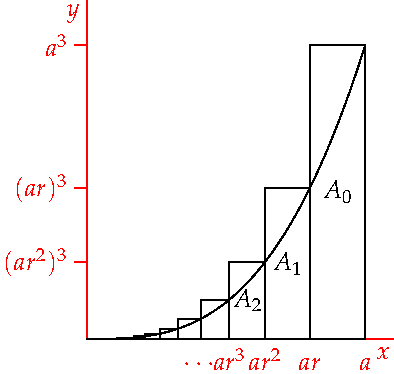
\includegraphics{analytic-fermat-area}
\end{minipage}
\medbreak

This is non-rigorous by modern standards and again implicitly invokes limits\footnote{%
	For Fermat, $r=\frac nm$ would have been rational, and he'd have set $m=n$ at the end as in his adequation method
}
by setting $r=1$. Regardless, Fermat is able to establish the power law $\int_0^a x^n\,\dx=\frac 1{n+1}a^{n+1}$ for any positive integer $n$.


\boldsubsubsection{Italian Calculus in the 17\th{} Century: the Area and Volume Problems}

In contrast to the work of Fermat and Descartes, contemporary Italian scholars were more focused on integration problems. Here is Galileo's classic `soup bowl' problem, where he compares the volume between a hemisphere and a cylinder to that of a cone.
\begin{center}
	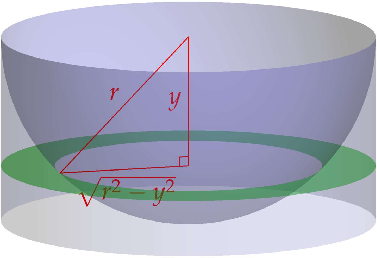
\includegraphics{analytic-soupbowl}
	\qquad\qquad
	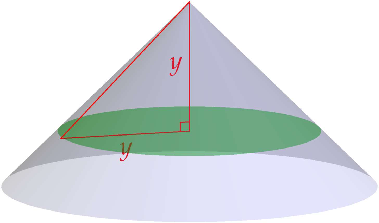
\includegraphics{analytic-soupbowl2}
\end{center}

Galileo observed\footnote{%
	As did Archimedes 1900 years earlier (pg.\,\pageref{pg:archmethod}), though Galileo was unaware of it.
}
that the \textcolor{Green}{cross-sectional areas} on both sides are equal (to $\pi y^2$). Since all cross-sections are equal, so must be the volumes. Unfortunately for Galileo, he couldn't sufficiently address two philosophical objections:
\begin{description}\itemsep0pt
  \item[\normalfont\emph{The zero-measure problem}] If cross-sections are `equal,' then the top cross-sections state that a circle `equals' a point.
  \item[\normalfont\emph{Infinitesimals sum to the whole?}] Can we claim that equal cross-sections imply equal volumes?
\end{description}
It was Galileo's advocacy on these points that first gained him notoriety with the Church. His later evangelism for the Copernican theory merely rekindled old animosities.


\boldinline{Bonaventura Cavalieri (1598--1647)}

Cavalieri, a student of Galileo and a Jesuat scholar, gave a more thorough discussion of indivisibles in 1635. He is particularly remembered for \emph{Cavalieri's principle}:\vspace{-5pt}

\begin{quote}
	If geometric figures have proportional cross-sectional measure at every point relative to a line, then the figures have measure in the same proportion.
\end{quote}

\begin{minipage}[t]{0.62\linewidth}\vspace{-10pt}
	Galileo's soup bowl is an example of this reasoning, where the `line' is any vertical.\smallbreak
	Another classic example involves sliding a stack of coins or a deck of cards; the volume of the slanted coin stack equals that of the cylinder.
\end{minipage}
\hfill
\begin{minipage}[t]{0.37\linewidth}\vspace{-10pt}
	\flushright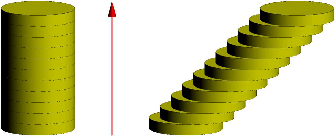
\includegraphics{analytic-cylinder}
\end{minipage}\medbreak
%In pure geometry, we could imagine a square having the same area as a parallelogram with the same height.\\

Extending his principle, Cavalieri inferred the power law $\int_0^ax^n\dx=\frac 1{n+1}a^{n+1}$, giving reasonable arguments for $n=1$ and 2. Here is a sketch of his approach for $n=2$.\par
\begin{minipage}[t]{0.68\linewidth}\vspace{0pt}
	Draw a cube of side $x$ inside a cube of side $a$. This consists of three congruent pyramids with base $a^2$ and eight $a$.\smallbreak
	Consider the pyramid apex $O$ and whose base is the square face nearest the viewer. The \textcolor{Green}{cross-section} of this pyramid at position $x$ has area $x^2$. In Cavalieri's language, the pyramid is `all the squares;' in modern language
	\[
		\int_0^ax^2\,\dx=\frac 13a^3
	\]
\end{minipage}
\hfill
\begin{minipage}[t]{0.3\linewidth}\vspace{-10pt}
	\flushright
\href{http://www.math.uci.edu/~ndonalds/math184/analytic-cavalieri.html}{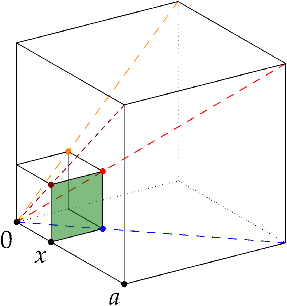
\includegraphics[scale=0.9]{analytic-cavalieri}}
\end{minipage}\medbreak

\phantomsection\label{pg:cavspiral}
Cavalieri also used his method (Book IV, Prop 19 of \emph{Geometria Indivisibilis}) to calculate the area enclosed in an \textcolor{red}{Archimedean spiral.} Suppose $B$ moves at constant speed along a line $\cl{OA}$ rotating at constant speed about $O$. In polar co-ordinates $B$ traces a curve $r=k\theta$ for $0\le\theta\le 2\pi$ (we take $k=1$).\par
\begin{minipage}[t]{0.73\textwidth}\vspace{-5pt}
	If $\nm{OB}=r$, then the \textcolor{blue}{arc} \emph{inside} the spiral has length
	\[
		\ell(r)=2\pi r\cdot\frac{2\pi-\theta}{2\pi}=r(2\pi-r)
	\]
	Imagine the \textcolor{blue}{arc} as a noodle which, when cut at $B$ and allowed to fall, forms the \textcolor{Green}{line} $\cl{CD}$. The area in the spiral therefore equals that within the parabola which (thanks to Archimedes and Cavalieri himself) is  $\frac 43$ that of the largest triangle that can fit inside, namely
	\[
		\frac 43\cdot \frac 12(2\pi)\ell(\pi)=\frac 43\pi^3
	\]
\end{minipage}
\hfill
\begin{minipage}[t]{0.25\textwidth}\vspace{-5pt}
	\flushright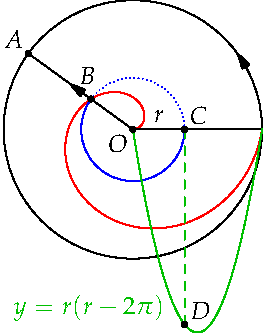
\includegraphics[scale=0.9]{cavalieri1}
\end{minipage}\medbreak

Cavalieri did this slightly differently, his parabola being drawn in a rectangle and the difference subtracted from a triangle, but the above is easier to visualize.\medbreak %(see \emph{Infinitessimal, pg 100})

Cavalieri did not court controversy like Galileo, being well-aware of the contentious nature of indivisibles and taking great pains to distinguish `all the lines/squares' of a figure from the figure itself. \emph{Geometria Indivisibilis} was dense and difficult, so it wasn't easy to challenge. Cavalieri therefore remained relatively safe, even as his political rivals (the Jesuit order) worked hard to stamp out the `dangerous' study of indivisibles.

\goodbreak

\boldinline{Evangelista Torricelli (1608--1647)} A contemporary of Galileo and Cavalieri, Torricelli made several applications of Cavalieri's principle and advocated for its careful use.

\begin{minipage}[t]{0.7\linewidth}\vspace{0pt}
	If the sides of a rectangle are in the ratio 2\,:\,1, so also are indicated red and blue segments. In Cavalieri's language, `all the lines' of the red triangle are twice `all the lines' of the blue triangle! Torricelli observes that the red triangle cannot have twice the area of the blue, since they are congruent and points out that Cavalieri's principle has been misapplied: the cross-sections were not measured with reference to a common line.
\end{minipage}
\hfill
\begin{minipage}[t]{0.29\linewidth}\vspace{0pt}
	\flushright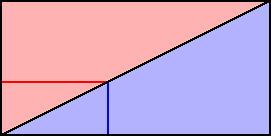
\includegraphics{analytic-torri1}
\end{minipage}\medbreak

In modern language, $\int_0^2\frac 12x\,\dx=\int_0^12y\,\dy$ are equal via the substitution $x=2y$. The point is that the infinitesimals are also in the \emph{same ratio} $\dx:\dy=2:1$.\bigbreak


Another of Torricelli's examples offers a seeming paradox.

\begin{minipage}[t]{0.58\linewidth}\vspace{-5pt}
	The hyperbola with equation $z=\frac 1x$ is rotated around the $z$-axis. A \textcolor{Green}{cylinder} centered on the $z$-axis with radius $x$ lying under the surface has surface area
	\[
		A=\text{circumference}\cdot\text{height}=2\pi xz=2\pi
	\]
	Underneath the graph at $x$, Torricelli draws a \textcolor{Green}{circular disk} with area $2\pi$. Since the area of this disk is independent of $x$, he argues that the volume under the original \textcolor{blue}{surface} out to radius $a$ equals the volume of the solid \textcolor{orange}{cylinder}:
	\[
		V=2\pi a
	\]
	Torricelli argues that this is a correct use of Cavalieri's principle since the cylindrical `cross-sections' and the circular cross-sections are both measured with respect to the same line (the $x$-axis).\smallbreak
	This is precisely the method of volume by cylindrical shells that we learn in modern calculus:
	\[
		V=\int_0^a 2\pi x\cdot\frac 1x\,\dx=2\pi a
	\]
	The conundrum is that the surface is \emph{infinitely tall}! How can we justify the idea that it lies above a \emph{finite} volume?
\end{minipage}
\hfill
\begin{minipage}[t]{0.41\linewidth}\vspace{-10pt}
	\flushright
	\href{http://www.math.uci.edu/~ndonalds/math184/analytic-torri2.html}{
		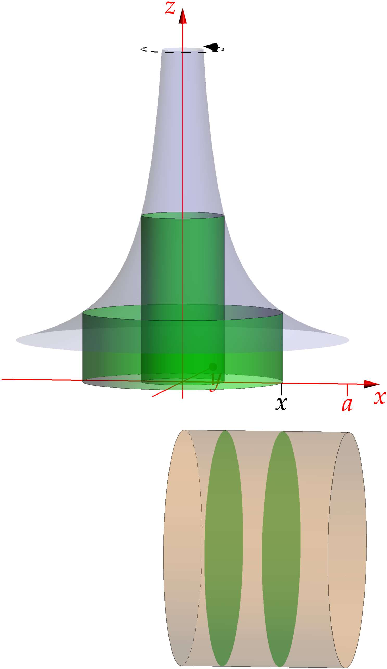
\includegraphics{analytic-torri2}
	}
\end{minipage}
\bigbreak

Galileo, Cavalieri and Torricelli mark the end of 400 years of Italian dominance of in science and mathematics dating back to Fibonacci. Their ideas were too controversial to thrive so close to the center of Church power. The center of European science and philosophy therefore moved northward. The English and French (protestant) reformations of the 1500s together with developing ideas of reformed government\footnote{%
	For instance Hobbes' \emph{Leviathan} written during the English Civil War (1642--1651) was a plea for the constraint of absolute monarchical power. The War itself indeed proved decapitatingly effective at reining in a King\ldots%
}
meant that Northern Europe provided more fertile ground for new ideas.
\goodbreak


\begin{exercises}{}{}
	\exstart Find the maximum of $p(x)=5+x-2x^2$ using Fermat's first method.
	
	\begin{enumerate}\setcounter{enumi}{1}
		\item%[15-4]* 
		Use Fermat's second method (``$+e$'') to find the maximum of $bx-x^3$. How might Fermat decide which of the two solutions to choose as his maximum?
	  
		\item%[15-5]*
		Justify Fermat's first method of determining maxima and minima by showing that if $M$ is a maximum of $p(x)$, then the polynomial $p(x)-M$ always has a factor $(x-a)^2$, where $a$ is the value of $x$ giving the maximum.
		
		
		\item Use Descartes' method of normals to compute the slope of the curve $y=x^2$ at $(a,a^2)$.
	
		\item Suppose the surface of a sphere of radius $r$ is subdivided into infinitesimal regions of equal area. Following Kepler, use the formula for the volume of a cone ($\frac 13$base$\cdot$height)	to find the relationship between the volume $V$ of the sphere and its surface area $A$.
			
	 	\item%[15-2]* 
	 	(A problem of Kepler)\lstsp Show that the largest circular cylinder that can be inscribed in a sphere is one in which the ratio of diameter to altitude is $\sqrt 2:1$.\par
	 	(\emph{Hint: Relate the problem to finding the maximum of the function $f(x)=x-\frac 14x^3$, for which you can use modern calculus})
		
		
	% 	\item%[15-22]*
	% 	Determine the area under the curve $y=px^k$ from $x=0$ to $x=x_0$ by dividing the interval $[0,x_0]$ into an infinite set of subintervals, beginning from the right with the points $a_0=x_0,\ a_1=\frac nmx_0,\ a_2=\left(\frac nm\right)^2x_0,\ldots$ where $n<m$, and proceeding as in Fermat's derivation of the area under the hyperbola.
	
	
		\item We consider a version of Gregory St.\,Vincent's 1647 approach to the area under the hyperbola $xy=1$.
		\begin{enumerate}
		  \begin{minipage}[t]{0.6\linewidth}\vspace{-3pt}
		  \item If $1<a<b$ and $r>0$ as in the picture, explain why the areas $A$ and $B$ under the curve satisfy the same inequalities
		  \[
		  	\frac{b-a}b<A,B<\frac{b-a}a
		  \]
		  (\emph{Since $[a,b]$ may be subdivided into arbitrarily many subintervals, the areas $A_1$ and $A_2$ are therefore equal}) 
		  \end{minipage}
		  \hfill
		  \begin{minipage}[t]{0.39\linewidth}\vspace{-15pt}
		  	\flushright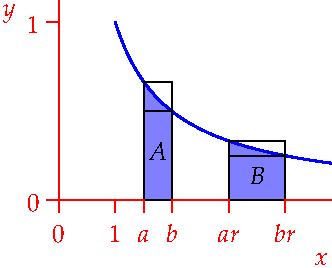
\includegraphics{analytic-stv-area}
		  \end{minipage}\par
		  
		  \item If $A(x)$ is the area under the hyperbola between 1 and $x$, explain why $A$ satisfies the \emph{logarithmic} identity
		  \[
		  	A(x_1x_2)=A(x_1)+A(x_2)
		  \]
		  Why are you not surprised by this?\par
		  (\emph{For simplicity, assume $1<x_1<x_1x_2$})
		\end{enumerate}
		
		\begin{minipage}[t]{0.6\linewidth}\vspace{0pt}
			\item Consider two copies of triangle with sides $a,b$ arranged into a rectangle. Argue that `all the lines' of the rectangle are twice `all the lines' of the triangle.\par
			(\emph{In modern language, $\int_0^ab\,\dy=2\int_0^a\frac bay\,\dy$}) 
		\end{minipage}
		\hfill
		\begin{minipage}[t]{0.39\linewidth}\vspace{0pt}
			\flushright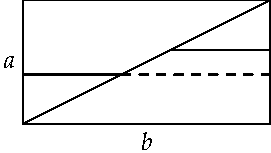
\includegraphics{analytic-torri3}
		\end{minipage}\par
		
		\item Repeat Cavalieri's analysis of the spiral (pg.\,\pageref{pg:cavspiral}) to find the area inside one revolution of the curve $r=k\theta$ for any $k>0$.
		
	\end{enumerate}
\end{exercises}


\clearpage




\subsection{Calculus in the late 1600s}\label{sec:calc2}

By the second half of the 17\th{} century, the mathematical center of Europe had moved northwards, to France, Germany, Holland and Britain. In this section we present some of this work, culminating with the efforts of Newton and Leibniz.\par

\begin{minipage}[t]{0.64\linewidth}\vspace{0pt}
	\boldinline{Hendrick van Heuraet (1634--1660)} Working in Holland, van Heuraet studied Descartes' and argued that the arc-length of a curve described by a function $y$ equals the area under the curve $z=\frac ny$ where $n$ is the `normal' curve. His method appeared in Frans van Schooten's 1659 version of Descartes' \emph{La Geometrie.} To see why this should make sense, recall Descartes' method of normals and observe that the ratio $n:y$ equals that of $\ds:\dx$ in a differential triangle.\smallbreak
	His most famous example involved calculating the arc-length of the curve $y^2=x^3$. By Descartes' method,
	\begin{gather*}
		\qquad
		\begin{cases}
			(x-a-\nu)^2+y^2=n^2\\
			y^2=x^3
		\end{cases}\\
		\begin{aligned}
			\implies 0&= x^3+x^2-2(x+\nu)x+(a+\nu)^2-n^2\\
			&=(x-a)^2(x+2a+1)+(3a^2-2\nu)x\\
			&\qquad\qquad +\nu^2+2a\nu-2a^3-n^2
		\end{aligned}
	\end{gather*}
\end{minipage}
\hfill
\begin{minipage}[t]{0.35\linewidth}\vspace{-4pt}
	\flushright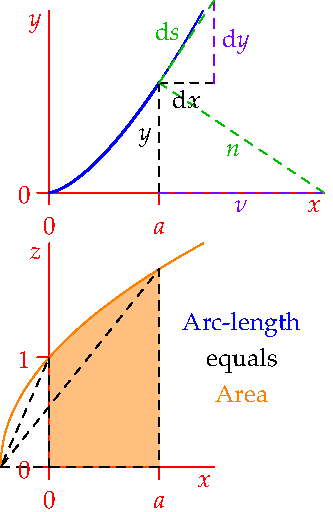
\includegraphics{calc-gregory}
\end{minipage}\medbreak

Since the remainder must be zero, we conclude that $\nu=\frac 32a^2$, from which
\[
	n=\sqrt{\nu^2+y^2}=\sqrt{\frac 94a^4+a^3}\implies z=\frac ny=\sqrt{\frac 94a+1}
\]
The \textcolor{blue}{arc-length} from $x=0$ to $a$ is therefore the \textcolor{orange}{area under the parabola} $z^2=\frac 94x+1$ between the same limits. By the usual Archimedean $\frac 43$-triangle approach, we see that
\[
	\text{\textcolor{blue}{Arc-length}}=\frac 43\left[\frac 12\cdot\left(\frac 49+a\right)z(a)-\frac 12\cdot \frac 49\cdot 1\right] =\left[a+\frac 49\right]^{3/2}-\frac 8{27}
\]

\boldinline{James Gregory (1638--1675)} Hailing from Aberdeen, Scotland, Gregory studied in Italy with Stefano Angeli, a pupil of Torricelli, before returning to Scotland where he became chair of mathematics at St.\,Andrews, and then Edinburgh.\smallbreak
Gregory repeats van Heuraet's work relating the length of a curve to the area under another, before considering whether the process can be reversed: given a curve $z(x)$, can we find a curve $y(x)$ such that the arc-length of $y$ is given by the area under $z$? In modern language, given $z$, find $y$ such that
\[
	\int_0^a\sqrt{1+y'^2}\,\dx=\int_0^az\,\dx
\]
which we'd view as solving the ODE $\diff[y]{x}=\sqrt{z^2-1}$. Gregory's solution was to \emph{define} $y$ to be the area under the curve $\sqrt{z^2-1}$ from $0$ to $a$. This is essentially part 1 of the fundamental theorem of calculus: if you want something whose slope (derivative) is given, define it to be the area under the curve!

\goodbreak

\boldinline{Isaac Barrow (1630--1677)} Like Gregory, Barrow also studied mathematics in Italy (and France), before returning to England to become the inaugural Lucasian Professor of Mathematics\footnote{%
	One of the most prestigious world-wide academic positions in \emph{theoretical Physics,} in large part due to the fame of its second incumbent: Issac Newton. Later chairs include Paul Dirac and Stephen Hawking.%
}
at Trinity College Cambridge. Barrow's work remained predominantly geometric; he stated proving geometric versions of both parts of the fundamental theorem, though credited Gregory with part of the argument. In a precursor of Newton's work, he also modified Fermat's algorithm for differentiation. For example, here is how Barrow would have found the slope of the curve $x^2+2xy^2=c$ at a point $(x,y)$:
\begin{itemize}\itemsep0pt
  \item Replace $x$ and $y$ with $x+e$ and $y+a$ respectively and expand:
  \[
  	x^2+2ex+e^2+2xy^2+4axy+2a^2x+2ey^2+4eay+2ea^2=c
  \]
  \item Delete everything from the original equation $x^2+2xy^2=c$ and every expression containing two or more of the terms $e,a$:
  \[
  	2ex+4axy+2ey^2=0
  \]
  \item Rearrange: the slope is the ratio $a:e=-x-y^2:2xy$
\end{itemize}
This is implicit differentiation, where $\dx=e$ and $\dy=a$. Note again the essential difficulty with these \emph{algorithmic} approaches to calculus: the infinitesimal quantities $e,a$ are necessary for the calculation, but most of them are discarded when no longer useful! Can we really calculate with objects that must simultaneously exist and be zero?\footnote{This is at the heart of Bishop George Berkeley's (after whom the Californian city and university are named) famous 1734 objection to calculus; that infinitesimals are merely the ``ghosts of departed quantities.''}


% 
% The idea is essentially the modern one. Suppose $y=f(x)$ is an increasing function and draw the differential triangle. The new area under the curve is then approximately $\Delta A\approx f(x)\dx$. That is $\diff[A]{x}=f(x)$ and the essential link between area and slope is established.\\




\boldsubsubsection{Isaac Newton (1642--1727)} 

The caricature of Newton is of an obsessive genius---difficult to get along with, but with a phenomenal ability to concentrate on problems. One possibly apocryphal story describes how he continued lecturing to an empty room even after no-one had turned up!\par

\begin{minipage}[t]{0.53\linewidth}\vspace{-4pt}
	We are mostly interested in Newton's mathematics, though his wider fame comes from its wide application, particularly to gravitation. In \emph{Philosophiæ Naturalis Principia Mathematica} (1686), Newton applied his three laws of motion\footnotemark{} and the machinery of calculus to prove the relationship between Kepler's laws of planetary motion (pg.\,\pageref{pg:keplerslaws}) and an inverse-square gravitational force. The \emph{Principia} is Newton's first published work involving calculus, though many of its results and his method appear to have been worked out 20 years previously, just after completing his undergraduate studies and while Cambridge was closed due to the 1665--6 plague epidemic.
\end{minipage}
\hfill
\begin{minipage}[t]{0.44\linewidth}\vspace{-5pt}
	\flushright
	\begin{tabular}{@{}c@{}}
		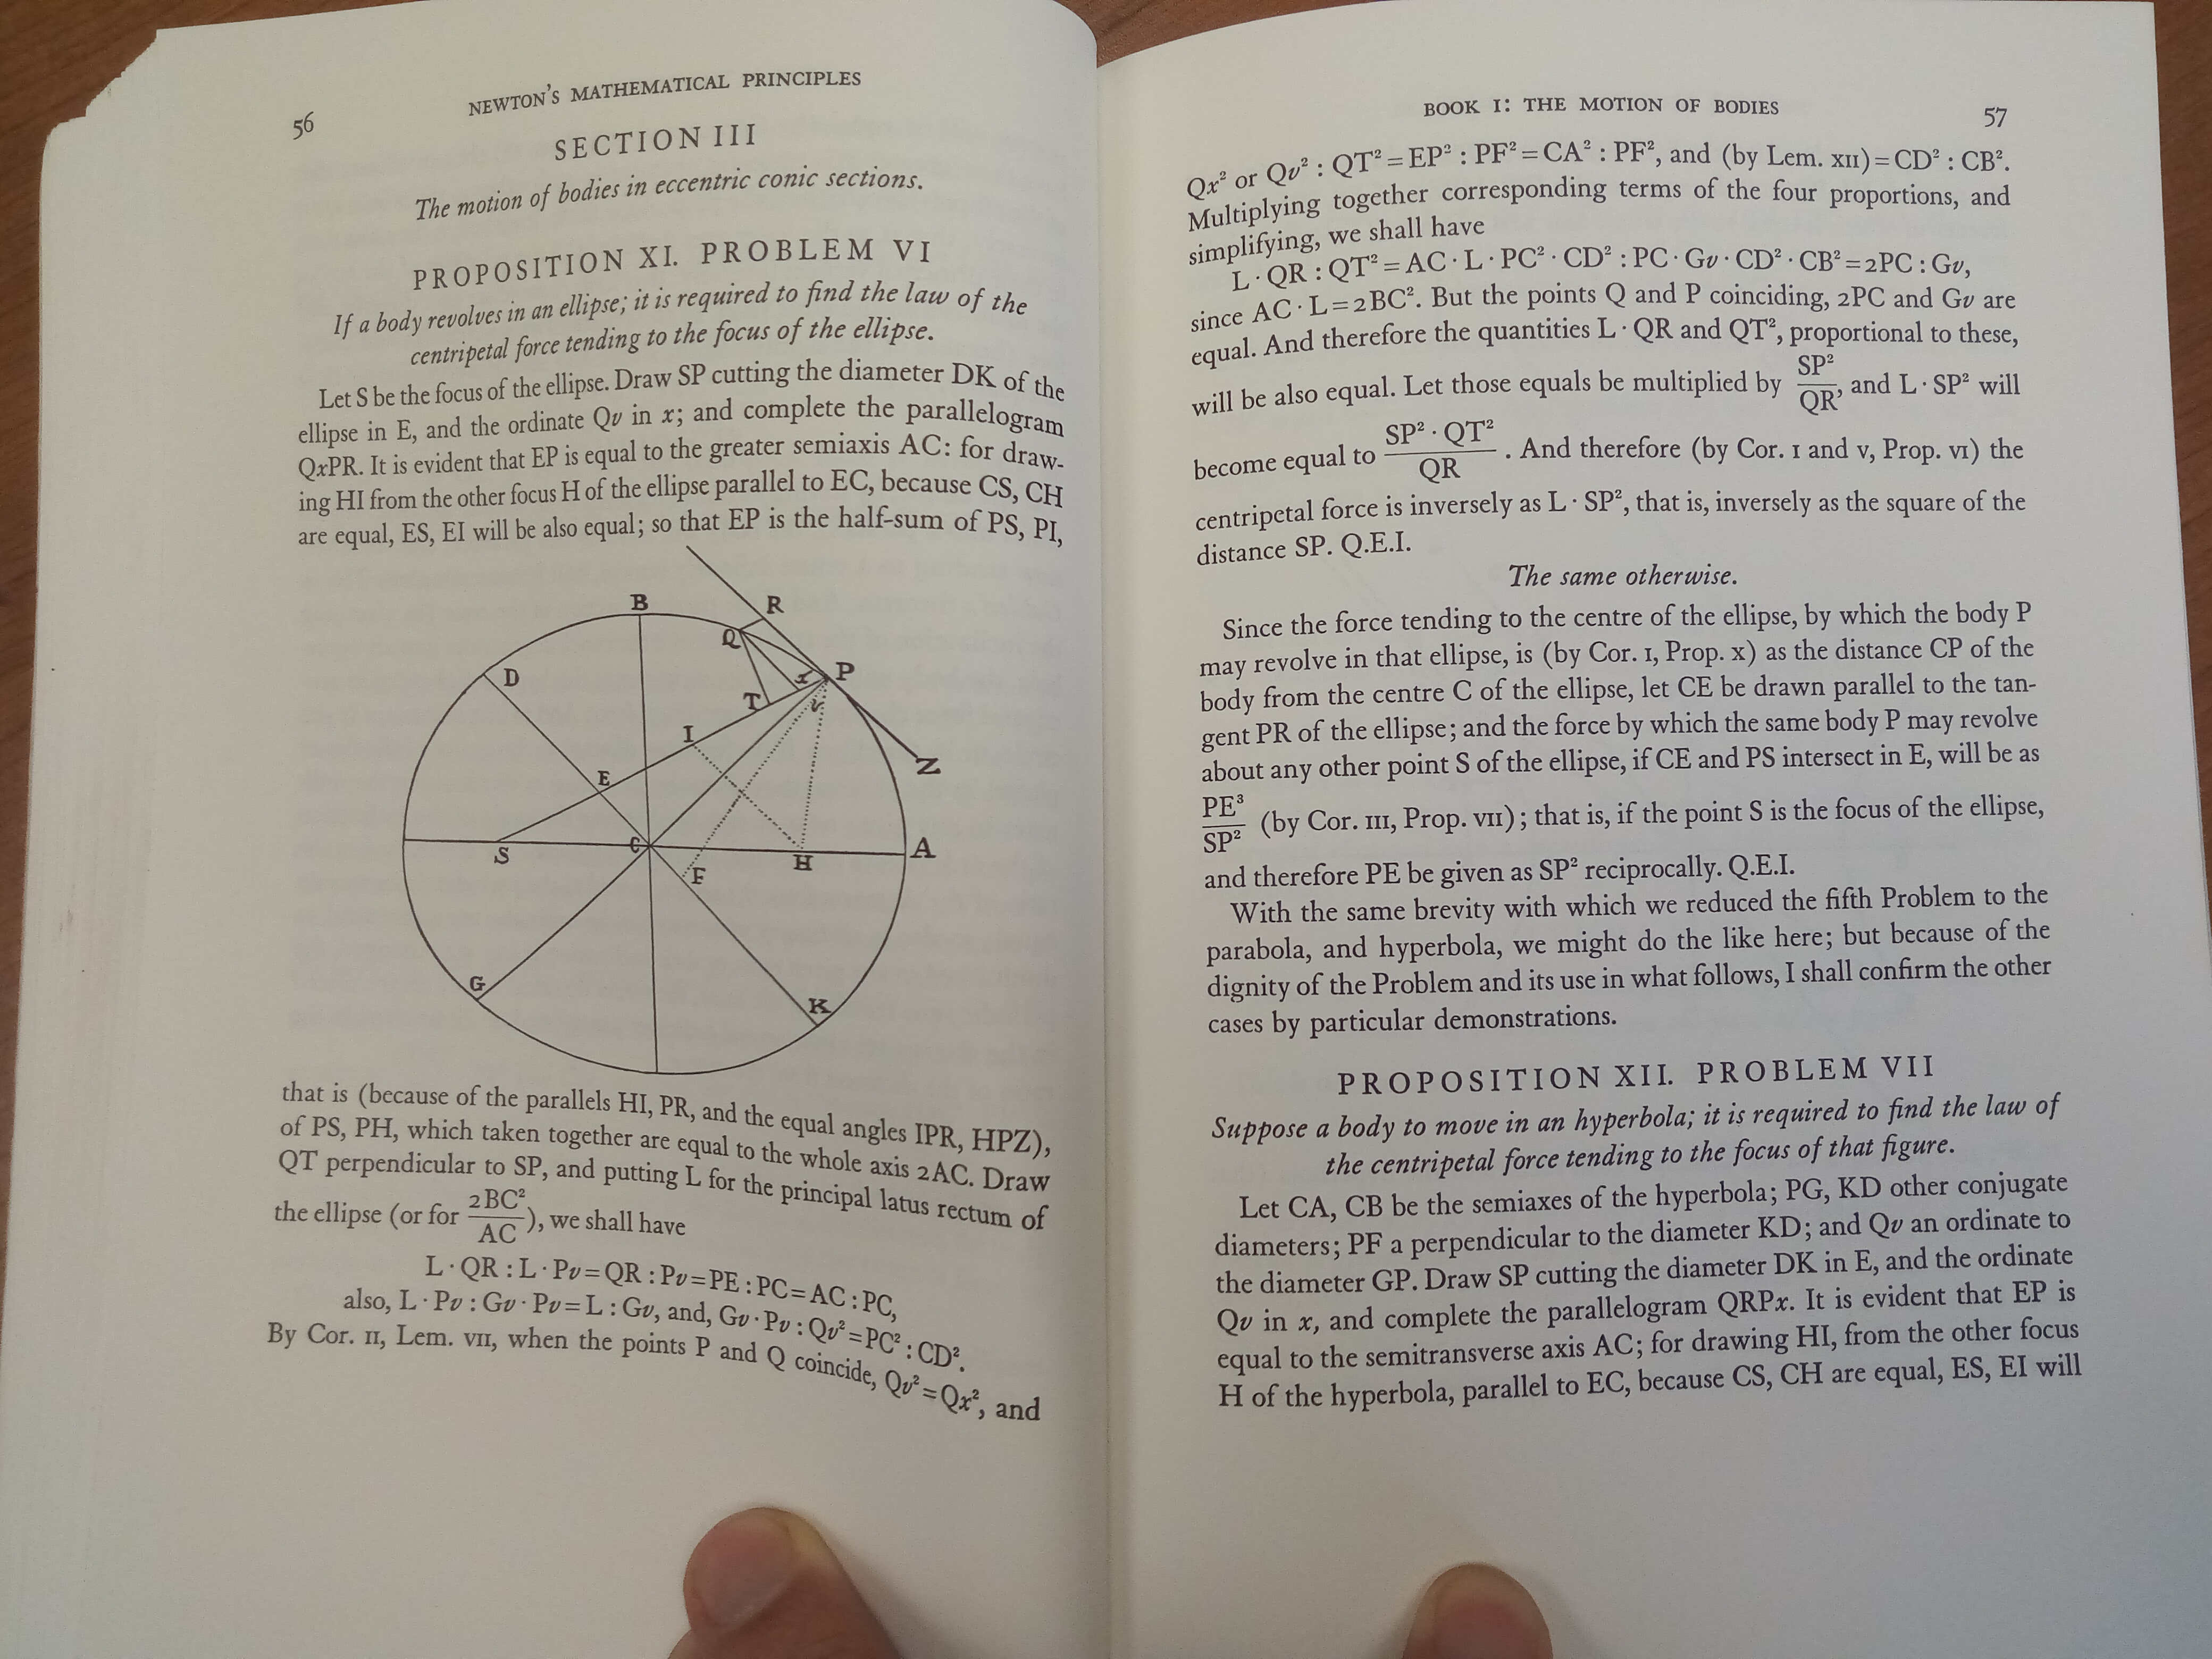
\includegraphics[width=\textwidth]{newton5.jpg}\\
		Kepler's 1st law $\implies$ inverse-square force
	\end{tabular}
\end{minipage}\smallbreak

\footnotetext{I.\,Inertial motion; \ II.\,$F=ma$; \ III.\,Equal-and-opposite forces. Consider these as the \emph{axioms} of Newtonian mechanics.}

\goodbreak
 
Newton's geometric presentation was typical for the time. He comments on how calculations are more efficient using indivisible methods, but that the `hypothesis of indivisibles seems somewhat harsh' (he likely wants to counter the impression that his method is philosophically shaky). Newton's approach makes it hard for modern readers to extract calculus algorithms; indeed the \emph{Principia} is not a calculus textbook and it is not really possible to learn calculus directly from it. Nevertheless, it contains notions of many standard concepts, for instance:
\begin{description}
	\item[Limits/continuity] Book I, Lemma I:\lstsp ``Quantities, \ldots which in any finite time converge continually to equality, and before the end of that time approach nearer to each other than by any given difference, become ultimately equal.''\par
One can see modern ideas appearing (e.g., $\forall \epsilon>0, \nm{a-b}<\epsilon\implies a=b$) though there is a long way to go! What, for instance does \emph{approach} mean?
	\item[Product Rule] In the following pages, Newton argues for the product rule by augmenting the sides of a rectangle.
	\begin{center}
		\begin{tabular}{ccc}
			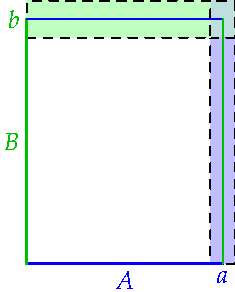
\includegraphics{newton-prodrule}
			&
			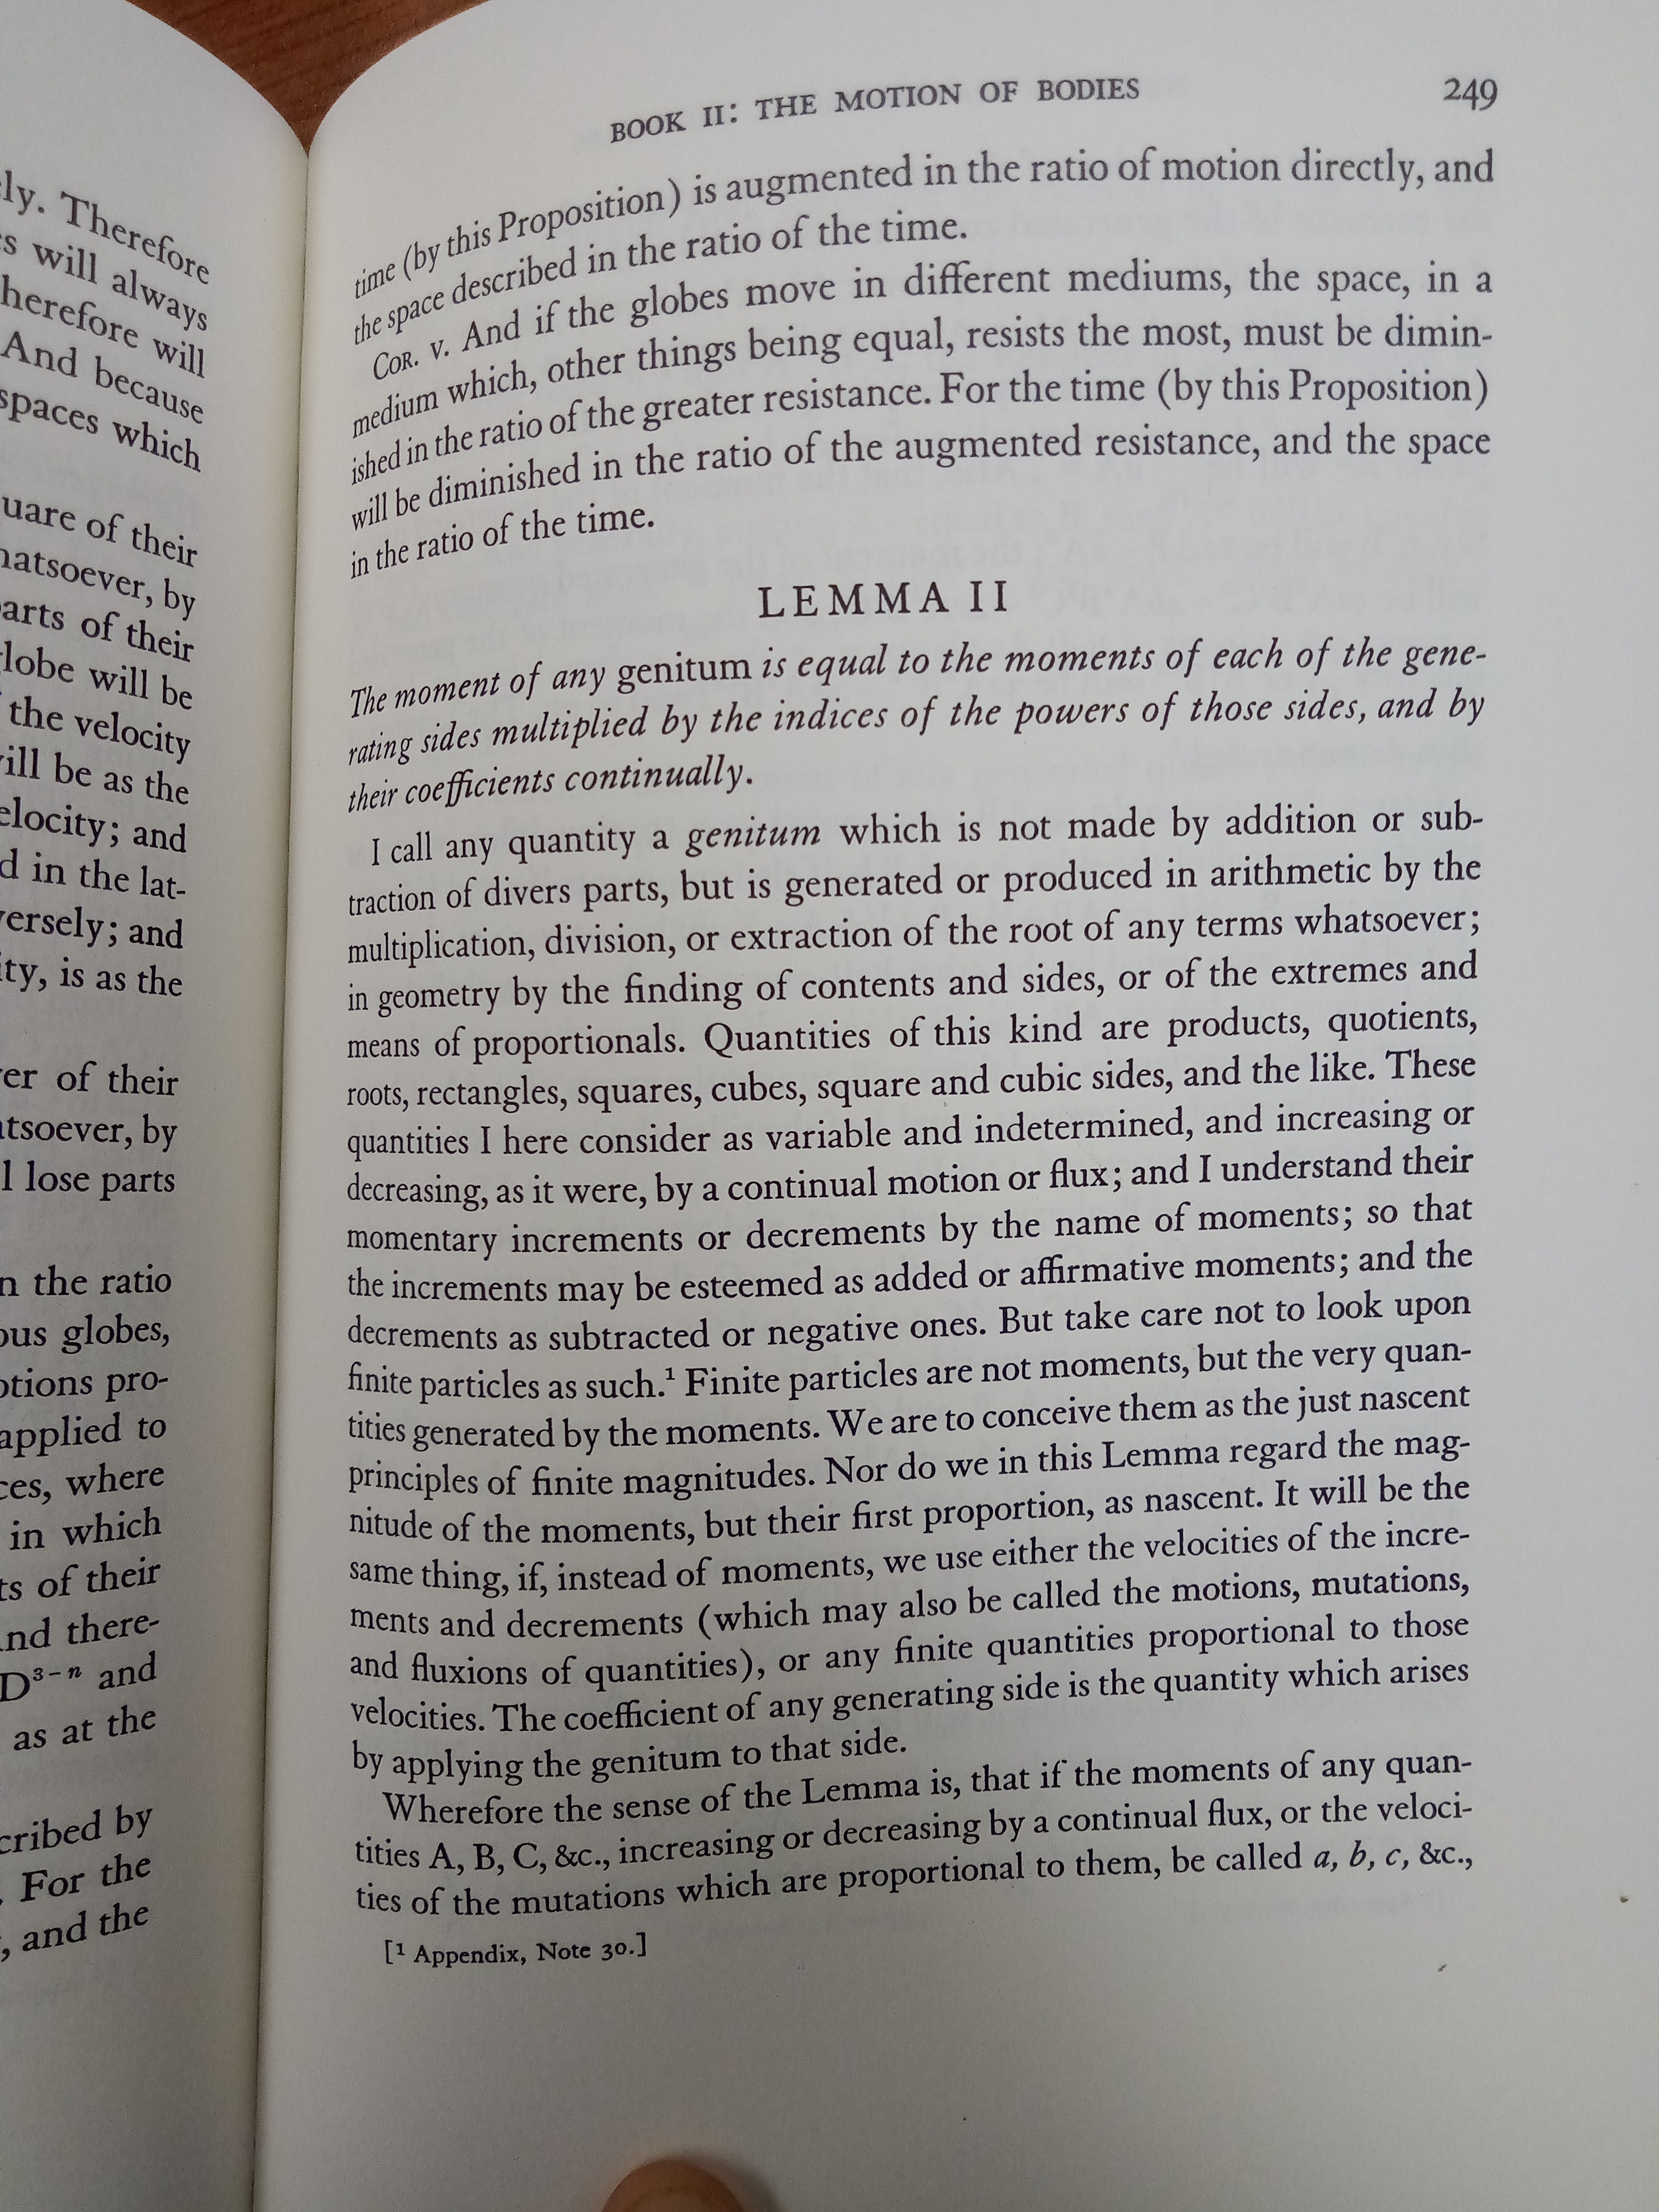
\includegraphics[height=140pt]{newton8.jpg}
			&
			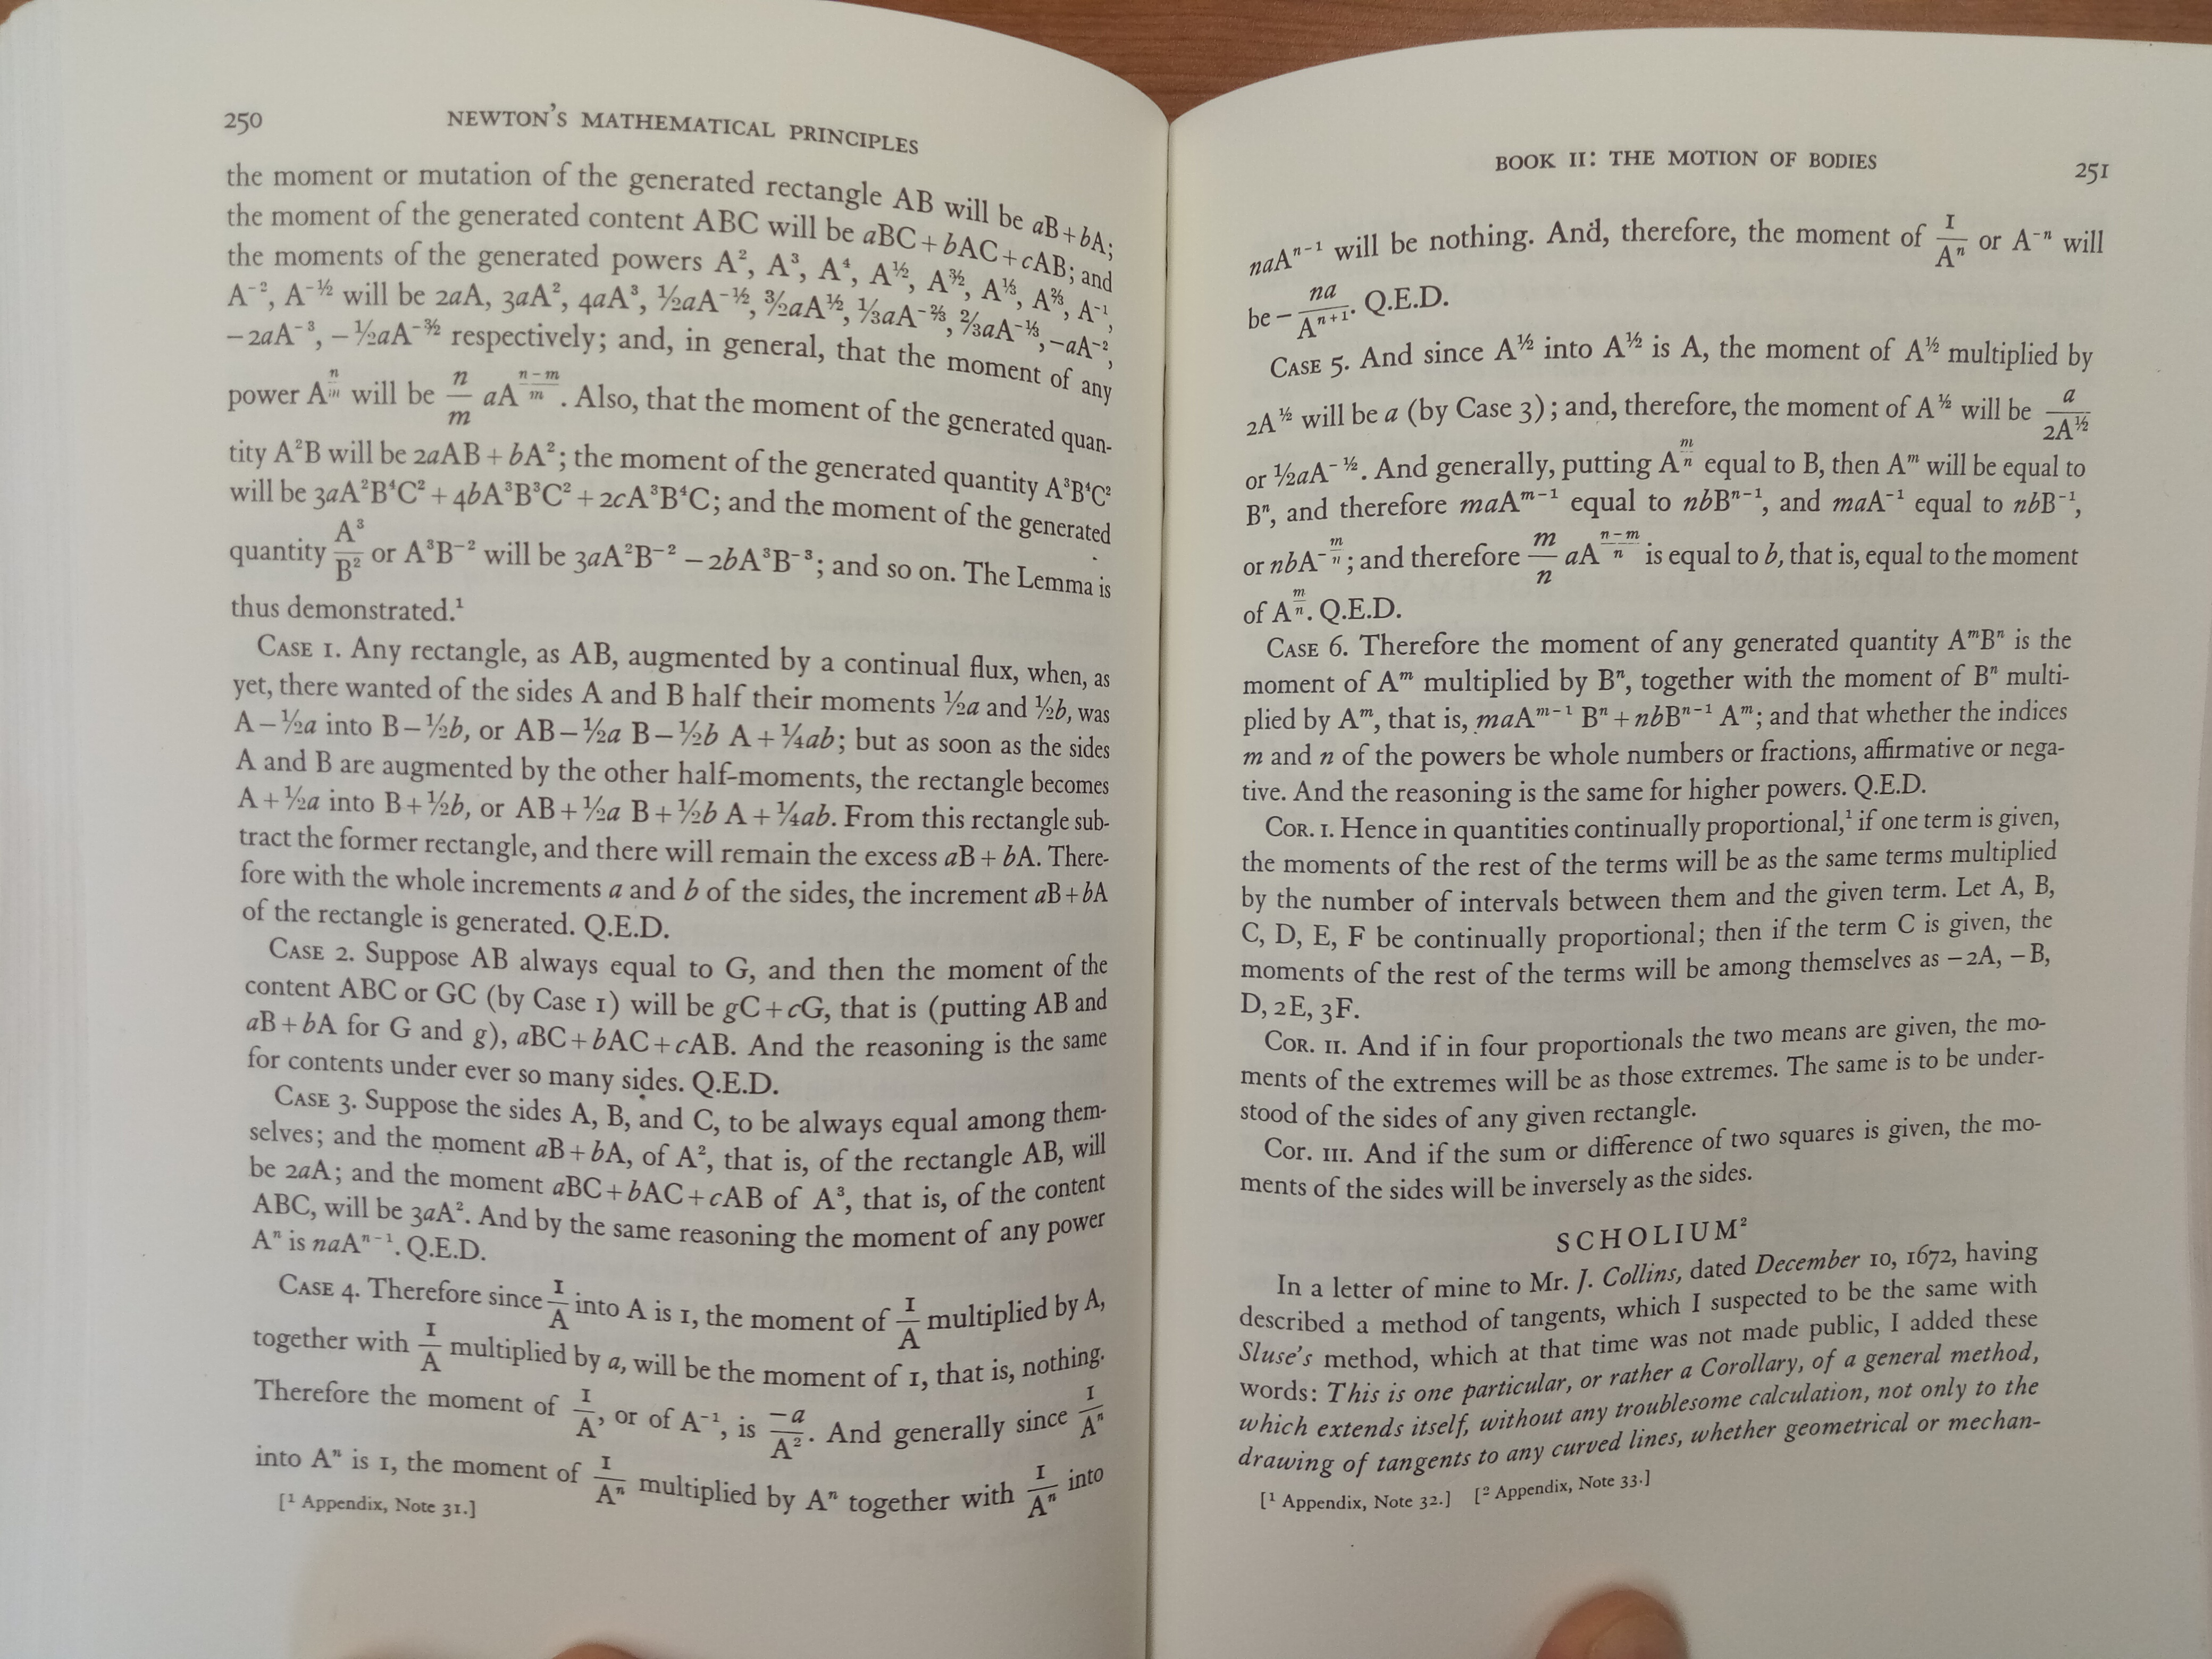
\includegraphics[height=140pt]{newton9.jpg}
		\end{tabular}
	\end{center}
	If $a,b$ are infinitesimal changes in the sides of a rectangle with sides $A,B$, then the \emph{moment of mutation} (infinitesimal change) of the generated rectangle $AB$ is the quantity $aB+bA$. In more familiar language,
	\[
		(A+a)(B+b)-AB\approx aB+bA
	\]
	where Newton ignores the double-infinitesimal quantity $ab$, exactly as did Barrow and others before him.
	\item[Power Law] In the same pages, Newton asserts the general power law for rational exponents 
	\begin{quote}
		\ldots the moment of any power $\displaystyle A^{\frac nn}$ will be $\displaystyle\frac nmaA^{\frac{n-m}m}$.
	\end{quote}
	in what seems like a non-rigorous appeal to induction based on the product rule. In reality, Newton established this using infinitesimal arguments; we'll see one of his methods for this shortly. 
\end{description}

In contrast to the mostly synthetic presentation in the \emph{Principia,} Newton made great use of algebra in his private calculations and correspondence with friends. Some of these private works were published many years later. We discuss some of his methods in what follows.


\goodbreak


\boldinline{Fluxions and Fluents} Newton's main language for calculus (he had several!) referred to time-dependent quantities $x,y$ as \emph{fluents} and their derivatives as \emph{fluxions,} denoted using dots $\dot x,\dot y$; the modern notation $y'$ comes from this.\footnote{%
	A fluent is a `flowing' quantity: to us, a \emph{smooth function,} though this was not formally defined. To be in \emph{flux} is to be changing, hence `rate of change.' Newton's dot-notation (`pricked letters') persists in the modern field of \emph{dynamics}: for instance $\ddot{\vr}=-\frac{GM}{r^3}\vr$ is the differential equation arising from Newton's second law together with the inverse-square law for gravitation (note the double dot for the second derivative).
}
Anti-derivatives were denoted by placing an accent directly over a quantity: $\acute{x}$ is a \emph{fluent of which $x$ is the fluxion.} Newton had several algorithms for computing fluxions, often variants of those of previous mathematicians: for instance, here he finds the relationship between the fluxions of fluents $x,y$ satisfying $x^2+3xy^3+y=5$.
\begin{itemize}\itemsep0pt
  \item Rearrange as a polynomial in $x$: thus $x^2+(3y^3)x+(y-5)=0$.
  \item Multiply terms by a decreasing arithmetic sequence (e.g.{} $2,1,0$) and the entire expression by $\frac{\dot x}x$:
  \[
  	(2x+3y^3)\dot x
  \] 
  \item Repeat for $y$, using the \emph{same arithmetic sequence}; in this example, 2 corresponds to $x^2$, so we start with 3 for $y^3$:
  \[
  	(3x)y^3+0y^2+y+(x^2-5)=0\rightsquigarrow (9xy^2+y)\dot y
  \]
  \item Sum these expressions, set equal to zero and rearrange for the required ratio:
  \[
  	(2x+3y^2)\dot x+(9xy^2+y)\dot y=0 \implies \frac{\dot y}{\dot x} = -\frac{2x+3y^2}{9xy^2+y}
  \]
\end{itemize}
The arithmetic sequence encodes the power law for derivatives, and the result is exactly what you'd expect from modern implicit differentiation.


\boldinline{The Binomial Series}

Also discovered during the plague years, but first appearing in a private letter of 1676, is Newton's discovery of the binomial series
\[
	(1+x)^\alpha=1+\sum_{k=1}^\infty\frac{\alpha(\alpha-1)(\alpha-2)\cdots(\alpha-k+1)}{k!}x^k
\]
which allowed Newton to expand expressions such as
\[
	(1+x)^{1/2} = 1+\frac 12x-\frac{1}{8}x^2 +\frac{1}{16}x^3 -\frac{5}{128}x^4 +\cdots
\]
Newton's version was only for fractional exponents and is more difficult to read:
\[
	P+PQ\ \frac mn=P\frac mn+\frac mnAQ+\frac{m-n}{2n}BQ+\frac{m-2n}{3n}CQ+\frac{m-3n}{4n}DQ+\cdots \tag{$\ast$}
\]
Newton wrote exponents using juxtaposition, and $A,B,C,D,\ldots$, meant `the previous term': thus $P\frac mn=P^{m/n}$, $A=P^{m/n}$ and $B=\frac mnAQ=\frac mnP^{m/n}Q$. In more modern language, ($\ast$) reads
\[
	(P+PQ)^{m/n}=P^{m/n}+\frac mn P^{m/n}Q +\frac{m(m-n)}{2n^2}P^{m/n}Q^2 +\frac{m(m-n)(m-2n)}{6n^3}P^{m/n}Q^3+\cdots
\]

\goodbreak

Newton's `proof' wouldn't pass modern muster. His discoveries were the result of some involved pattern-spotting! Several examples were explicitly verified by multiplying out or using long-division. For instance the series for $\sqrt{1+x}$ may be obtained
\begin{align*}
	&1+x=(1+ax+bx^2+cx^3+\cdots)^2=1+2ax+(a^2+2b)x^2+(2c+2ab)x^3+\cdots\\
	\implies &a=\frac 12,\quad b=-\frac 12a^2=-\frac 18,\quad c=-ab=\frac 1{16},\quad\text{etc.}\\
	\implies &\sqrt{1+x}=1+\frac 12x-\frac 18x^2+\frac 1{16}x^3+\cdots
\end{align*}
Newton did not work through the full theory of infinite series as you would encounter in a typical undergraduate analysis course. For instance:
\begin{itemize}
  \item $\sqrt{1+x}$ is well-defined for $x\ge -1$, yet the resulting series only converges when $-1\le x\le 1$. What happens in general: must a series converge to the original/generating function?
  \item Is it legitimate to differentiate and integrate power series term-by-term as if they are polynomials? Answer: (mostly) yes, though it was 150 years before Cauchy, Weierstraß and others could rigorously confirm this.
\end{itemize}



\boldinline{The Power Law \& the Fundamental Theorem}\phantomsection\label{pg:newtonpowerlaw}

Newton's ability to expand expressions as infinite series was essential to his arguments. Here is one of his arguments to prove the power law.
\begin{enumerate}
  \begin{minipage}[t]{0.68\linewidth}\vspace{-5pt}
	  \item Assume that the area under a curve $y$ is given by a function
	  \[
	  	z=\frac{x^{\frac mn+1}}{\frac mn+1}=\frac n{m+n}x^{\frac{m+n}n}
	  \]
	  \item If $x$ is increased by an infinitesimal amount $o$, then the new area under the curve is found using the binomial series
  \begin{align*}
  	\textcolor{Green}{z}+\textcolor{violet}{oy}&=\frac n{m+n}(x+o)^{\frac{m+n}n} =\frac n{m+n}x^{\frac{m+n}n}\left(1+\frac ox\right)^{\frac{m+n}n}\\
  	&=\frac n{m+n}x^{\frac{m+n}n} \Bigl(1+\frac{m+n}n\cdot\frac ox+\frac{(m+n)m}{2n^2}\cdot\frac{o^2}{x^2}+ \makebox[0pt][l]{$\cdots\Bigr)$}
  \end{align*}
	\end{minipage}
	\hfill
	\begin{minipage}[t]{0.31\linewidth}\vspace{-5pt}
		\flushright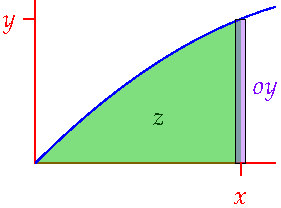
\includegraphics[scale=1]{ftcold}\vspace{-25pt}
	\end{minipage}\par
  


  \item Following Barrow, Newton cancels the terms in the original equation, divides by $o$, and throws out all remaining $o$-terms. The result is
  \[
  	y=\frac n{m+n}x^{\frac{m+n}n}\frac{m+n}n\cdot\frac 1x=x^{m/n}
  \]
  Note the essential with the fundamental theorem, which is intuitively obvious when $y$ is a `flowing' (continuous) quantity: the \textcolor{violet}{additional area} is approximately an infinitesimal rectangle $\textcolor{violet}{oy}=\dz$ with base $o=\dx$ and height $y$, whence
  \[
 		\textcolor{violet}{\dz}=y\,\dx \leftrightsquigarrow\diff[z]{x}=\diff x\int^xy(t)\,\dt=y(x)
  \]
\end{enumerate}

Using similar approaches, Newton produced one of the first tables of integrals, listing much of what you'd find inside the covers of an undergraduate calculus textbook! He also obtained power series for trigonometric and logarithmic functions, partly following the work of Gregory and others. By combining his approach with the power law, he was able to efficiently integrate and differentiate an enormous variety of functions.\smallbreak



\goodbreak



\boldsubsubsection{Gottfried Wilhelm Leibniz (1646--1716)}

Leibniz hailed from Leipzig, southwest of Berlin, in what was then part of the Holy Roman Empire. His initial studies were in philosophy, following his professor father. Though he eventually became a diplomat and then counsellor to the Duke of Hanover, his taste for advanced mathematics was fueled during his 1672--76 sojourn in Paris, where he was introduced to van Shooten's expansion of Descartes' geometric ideas, in particular the concept of the \emph{differential triangle} (page \pageref{sec:calc2}) which was already in use by others such as Pascal and Barrow.\smallbreak

The familiar notations for derivatives $\diff[y]{x}$ and integrals $\int y\,\dx$ come from Leibniz. Very loosely, here is its origin and how it relates to the fundamental theorem. Suppose that
\[
	(x_0,z_0),(x_1,z_1),\ldots,(x_n,z_n),\qquad x_0<x_1<\cdots<x_n
\]
describe a sequence of points along a curve $z(x)$ defined on an interval $[x_0,x_n]$. One may then form the sequences of \emph{differences} and \emph{sums} of the ordinates $z_i$:
\begin{gather*}
	\bigl(\delta z_i\bigr)=\bigl(z_1-z_0,\ z_2-z_1,\ \ldots,\ z_n-z_{n-1}\bigr),\qquad
	\bigl(\sum z_i\bigr) =\bigl(z_0,\ z_0+z_1,\ \ldots,\ z_0+\cdots+z_n\bigr)
\end{gather*}
Two relationships between sums and differences are immediate:
\begin{enumerate}
	\item The difference sequence of the sums returns the original sequence:
	\[
		\bigl(\delta\sum z_i\bigr)=\bigl(z_0,z_1,\ldots,z_n\bigr)
	\]
	\item The sum of the difference sequence is the net change in the ordinate:
	\[
		\sum\bigl(\delta z_i\bigr)=(z_1-z_0)+(z_2-z_1)+\cdots +(z_n-z_{n-1}) =z_n-z_0
	\]
\end{enumerate}
Leibniz's notation arises from viewing a curve as an \emph{infinite sequence} of points: he writes $\dz$ for the infinitesimal \emph{differences} and $\int$ for the \emph{sum} of infinitely many infinitesimal objects. Observation 2 becomes $\int \dz=z$: the sum of the infinitesimal changes in $z$ is the net change in $z$.\par
By assuming that $z(x)$ describes the \emph{area}\footnote{Notation is chosen to match Newton's discussion of the power law (page \pageref{pg:newtonpowerlaw}).} under a curve $y(x)$, Leibniz used the fact that $\dz=y\,\dx$ to write the area in the modern form $z=\int y\,\dx$. Our observations are now the two parts of the fundamental theorem of calculus!
\begin{enumerate}
  \item $\D\int y\,\dx=y$: the infinitesimal change in the area under the curve $y(x)$ equals the ordinate $y$.
  \item $\int y\,\dx=z$: the area under the curve is the sum of its infinitesimal increments.
\end{enumerate}
While we are happy to refer to infinitesimals and infinite sums, Leibniz was more cagey in his publications out of fear of criticism. He referred to each $\dx$ as an arbitrary (if small) \emph{finite} line segment, and therefore---like every other contemporary practitioner of calculus---fails to get to grips with the essential paradoxes involved. Regardless, he and his followers became adept at manipulating differential expressions. For instance, if $y=z^3+2z$, Leibniz might compute
\begin{align*}
	\dy&=(z+\dz)^3+2(z+\dz) -z^3-2z = 3z^2\,\dz+3z(\dz)^2 +(\dz)^3+2\,\dz\\
	&=(3z^2+2z)\,\dz
\end{align*}
where the $(\dz)^2$ and $(\dz)^3$ terms are discarded due to their (relatively) infinitesimal size. Using such approaches Leibniz justified general formulas such as the linearity of derivatives, the product, quotient and power rules. Even the chain rule is easy in Leibniz's notation: given $y(x)=\sqrt{1+x^3}$, Leibniz might perform a substitution $u=1+x^3$ and observe that
\[
	\dy=\D\sqrt u =\frac{\du}{2\sqrt u} =\frac{3x^2\,\dx}{2\sqrt{1+x^3}}
\]

Like Newton, Leibniz work extensively with power series. As a final example here is his computation of that for sine. In contrast to Newton's approach,\footnote{Newton first found a series for arcsine before computing its inverse.} Leibniz derived the well-known second-order ODE satisfied by sine.\par
\begin{minipage}[t]{0.7\linewidth}\vspace{-4pt}
In a circle of radius 1, let $s$ be the polar angle and $y=\sin s$ the ordinate. By considering the differential triangle, we see that
\[
	\frac{\dy}{\ds} =\sqrt{1-y^2} \implies (1-y^2)(\ds)^2=(\dy)^2 \tag{$\ast$}
\]
Leibniz supposes that infinitesimals $\ds$ describing the arc are constant and applies $\D$ again (with the product rule):\footnotemark
\[
	-2y\,(\dy)(\ds)^2=2(\dy)\D(\dy) \implies \frac{\D(\dy)}{(\ds)^2}=-y \quad \left(=\diff[^2y]{s^2}\right)
\]
\end{minipage}
\hfill
\begin{minipage}[t]{0.29\linewidth}\vspace{-8pt}
	\flushright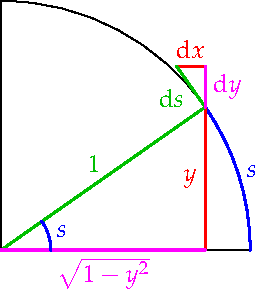
\includegraphics{leibniz-sine}
\end{minipage}\medbreak


\footnotetext{We've bracketed everything. When these are removed, we obtain the standard Leibniz notation for second derivatives!}

He then writes $y(s)=\sin s=c_0+c_1s+c_2s^2+c_3s^3\cdots$ as a power series. Since at $s=0$, $y=\sin s=0$ and $\ds=\dy$ (by $\ast$), Leibniz sees that $c_0=0$ and $c_1=1$. He now differentiates twice and equates coefficients:
\begin{align*}
	&2c_2+6c_3s+12c_4s^2+20c_5s^3+30c_6s^4+\cdots =-s-c_2s^2-c_3s^3-c_4^4-\cdots\\
	\implies &0=c_2=c_4=c_6=\cdots,\quad c_3=-\frac 16,\quad c_5=-\frac 1{20}c_3=\frac 1{120},\ \ldots 
\end{align*}
to obtain the familiar series
\[
	y=\sin s=s-\frac 16s^3+\frac 1{120}s^5+\cdots =s-\frac 1{3!}s^3+\frac 1{5!}s^5-\frac 1{7!}s^7+ \cdots
\]
While not precisely the same as modern calculus---in particular, the differentials $\dx,\dy,\ds$ are separate quantities---this should all seem very familiar! The computational efficiency of such notation super-charged mathematics and its applicability to real-world problems.

\goodbreak

\begin{exercises}{}{}
\exstart%[15-26]
  Show that to find the length of the arc of the parabola $y=x^2$ one needs to determine the area under the hyperbola $y^2-4x^2=1$.
\begin{enumerate}\setcounter{enumi}{1}
	\item%[15-28]
	Use Barrow's $a,e$ method to determine the slope of the tangent line to the curve $x^3+y^3=c^3$.
	
	\item%[16-2]
	Calculate a power series for $\frac 1{1-x^2}$ by using long-division.
	
	\item Use the binomial series to obtain a power series expression for $\ln(1+x)$, which Newton knew to describe the area under the curve $\frac 1{1+x}$. 

	
	\item Using his calculus, Newton was able to extend older methods of approximation.\par
	\begin{minipage}[t]{0.72\linewidth}\vspace{-5pt}
		\begin{itemize}\itemsep0pt
		  \item Suppose $f(c)=0$ and that $a_0$ is an initial approximation to $c$.
		  \item The tangent line at $\bigl(a_0,f(a_0)\bigr)$ has equation
		  \[
		  	y=f(a_0)+f'(a_0)(x-a_0)
		  \]
		  which intersects the $x$-axis at $a_1:=a_0-\frac{f(a_0)}{f'(a_0)}$.
		  \item Iterate to obtain a sequence $(a_n)$ that (typically) converges to $c$:
		  \[
		  	a_{n+1}=a_n-\frac{f(a_n)}{f'(a_n)}\quad \lim_{n\to\infty}a_n=c
		  \]
		\end{itemize}
	\end{minipage}
	\hfill
	\begin{minipage}[t]{0.27\linewidth}\vspace{-5pt}
		\flushright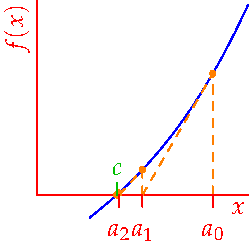
\includegraphics{newtonsmethod}
	\end{minipage}\par
	\begin{enumerate}
	  \item If $f(x)=x^2-c$, show that Newton's method is the ancient Babylonian method of the mean.
% If $f(x)=x^2-c$, this is the ancient Babylonian method of the mean:
% \[
% 	a_{n+1}=a_n-\frac{a_n^2-c}{2a_n}=\frac{a_n^2+c}{2a_n} =\frac 12\left(a_n+\frac c{a_n}\right)\xrightarrow[n\to\infty]{} \sqrt c
% \]
% The advantage of Newton's method is that it can be used to approximate roots for a much larger class of functions. For example, if $f(x)=x^3+2x-1$, then $f'(x)=3x^2+2$: if $a_0=1$, then
% \[
% 	a_{n+1}=a_n-\frac{a_n^3+2a_n-1}{3a_n^2+2} =\frac{2a_n^3+1}{3a_n^2+2} \implies (a_n)=(1,\tfrac 35,\tfrac{179}{385},\ldots)
% \]
		\item%[16-4]
		Use Newton's method to solve the equation $x^2-2=0$ to a result accurate to eight decimal places. How many steps does this take?
		%\item Compare this to the Chinese square-root algorithm.
	\end{enumerate}

	

	
% 	\item[16-6] Let $\frac 15y^5-\frac 14y^4+\frac 13y^3-\frac 12y^2+y-z=0$ and try $y=z$ as a first approximation. Then
% 	\[\frac 15z^5-\frac 14z^4+\frac 13z^3-\frac 12z^2=0\tag*{($\ast$)}\]
% 	Now try $y=z+p$.Then
% 	\begin{gather*}
% 	0=\frac 15z^5+pz^4-\frac 14z^4-pz^3+\frac 13z^3+pz^2-\frac 12z^2-pz+p+\text{non-linear terms in $p$}
% 	\end{gather*}
% 	after cancelling non-linear terms in $p$. At ths point the question is a little cryptic. Since we want $p$ to be a multiple of $z^2$, we follow the approach of question 5 and delete all terms of order higher than 2 in $z$. The result is
% 	\[0=-\frac 12z^2+p\implies p=\frac 12z^2\]
% 	It is perhaps easier to follow, if more difficult to calculate, by trying a new substitution $y=z+\frac 12z^2+az^3$. Substituting into the original equation and cancelling all terms in $a$ higher than 1 or $z$ higher than 3, we obtain
% 	\begin{align*}
% 	0&=\frac 15\left(z+\frac 12z^2+az^3\right)^5-\frac 14\left(z+\frac 12z^2+az^3\right)^4+\frac 13\left(z+\frac 12z^2+az^3\right)^3\\
% 	&\qquad\qquad-\frac 12\left(z+\frac 12z^2+az^3\right)^2+\left(\frac 12z^2+az^3\right)\\
% 	&=\frac 13z^3-\frac 12(z^2+z^3)+\left(\frac 12z^2+az^3\right) =-\frac 16z^3+az^3\implies a=\frac 16
% 	\end{align*} 
% 	The next approximation is therefore $z+\frac 12z^2+\frac 16z^3$. A similar approach yields the next term $\frac 1{24}z^4$.
	
	\item%[16-8]
	Calculate the relationship of the fluxions in the equation $x^3-ax^2+axy-y^3=0$ using multiplication by the progression 4, 3, 2, 1. Compare to what happens if you use the progression 3, 2, 1, 0. What do you notice?
	
	
	\item Use Leibniz's differential triangle to argue that
	\[
		x=\cos s\quad\text{and}\quad \dx=-y\,\ds
	\]
	Where does the negative sign come from? Hence find the standard power series representation for cosine and conclude that the rate of change (derivative) of sine is cosine.
	

	\item%[16-24] modified
	Given a curve $y(x)$ with $y(0)=0$, Leibniz's \emph{transmutation theorem} relates the area under $y$ and the curve $z(x)=y-x\diff[y]{x}$ obtained by considering the $y$-intercepts of the tangent lines to the original:
	\[
		\int_0^a y\,\dx=\frac 12\left[ay(a)+\int_0^a z\,\dx\right]
	\]
	If $x^p=y^q$, find $z$ and use the transmutation theorem to find the area $\int_0^a y\,\dx$.\par
	How does the transmutation theorem relate to \emph{integration by parts}?
	
% 	\item%[16-24]
% 	Given the curve $y^q=x^p$ ($q>p>0$), show using the transmutation theorem that 
% 	\[\int_0^{x_0}y\dx=\frac{qx_0y_0}{p+q}\]
% 	Note that from $y^q=x^p$, it follows that $\frac qy\dy=\frac px\dx$, and therefore that $z=y-x\diff[y]{x}=\frac{q-p}qy$.
	
	

\end{enumerate}
\end{exercises}


%BIG ideas: 1) algebra kills geometry. 2) expansion of the idea of number from $\N$ to $\R$

%Etymology: Calculus (single pebble) is the origin of `calculation.' Prior to N/L used for any mathematical algorithmic technique (algebraic calculus). Heirs to N/L referred to their methods as `infinitesimal calculus,' from which the first term was eventually dropped. 
